\documentclass[
  12pt,
  a4paper,
  oneside,
  brazilian,
  sumario=tradicional
]{abntex2}

% ============================================================
%  CORREÇÃO DO IDIOMA (evita aviso do babel)
% ============================================================
\PassOptionsToPackage{brazilian}{babel}

% ============================================================
%  PACOTES BÁSICOS (conforme ISPTEC/ABNT)
% ============================================================
\usepackage[T1]{fontenc}
\usepackage[utf8]{inputenc}
\usepackage{times}

% ============================================================
%  TÍTULOS EM TIMES NEW ROMAN
% ============================================================
\renewcommand{\ABNTEXchapterfont}{\rmfamily\bfseries}
\renewcommand{\ABNTEXchapterfontsize}{\Large}
\renewcommand{\ABNTEXsectionfont}{\rmfamily\bfseries}
\renewcommand{\ABNTEXsubsectionfont}{\rmfamily\bfseries}
\renewcommand{\ABNTEXsubsubsectionfont}{\rmfamily\bfseries}
\renewcommand{\ABNTEXsubsubsubsectionfont}{\rmfamily\bfseries}

% ============================================================
%  LAYOUT E ESPAÇAMENTOS (MARGENS ISPTEC)
% ============================================================
\usepackage{geometry}
\usepackage{setspace}
\usepackage{indentfirst}
\usepackage{emptypage}

\geometry{
  a4paper,
  left=3cm,
  right=2cm,
  top=3cm,
  bottom=2cm
}

\setlength{\parindent}{1.25cm}
\setlength{\parskip}{0pt}
\OnehalfSpacing
\sloppy

% ============================================================
%  TABELAS, FIGURAS E ILUSTRAÇÕES
% ============================================================
\usepackage{graphicx}
\usepackage{booktabs}
\usepackage{longtable}
\usepackage{array}
\usepackage{multirow}
\usepackage{float}
\usepackage{caption}
\usepackage{tikz}
\usetikzlibrary{positioning, arrows.meta, shapes, patterns, decorations.pathmorphing, calc}

% ============================================================
%  MARCADORES DE IMAGEM (placeholder simples)
%  Substitua cada \fbox por \includegraphics quando tiver a imagem real.
% ============================================================

\captionsetup{
  font=small,
  labelfont=bf,
  justification=centering,
  skip=6pt
}
\renewcommand{\fonte}[1]{\vspace{2pt}\par\noindent\footnotesize Fonte: #1}

% ============================================================
%  MATEMÁTICA
% ============================================================
\usepackage{amsmath}
\usepackage{amssymb}
\usepackage{amsfonts}

% ============================================================
%  UTILITÁRIOS
% ============================================================
\usepackage{hyperref}
\usepackage{xcolor}
\usepackage{enumitem}
\usepackage{lastpage}
\usepackage{epigraph}
\usepackage{microtype}

% ============================================================
%  CITAÇÕES ABNT (BibTeX) – estilo autor-ano
% ============================================================
\usepackage[alf,
  abnt-etal-list=0,
  abnt-etal-cite=3,
  abnt-repeated-author-omit=yes,
  abnt-emphasize=bf
]{abntex2cite}

% ============================================================
%  LINKS (PRETOS)
% ============================================================
\hypersetup{
  pdftitle={A história da Engenharia de Reservatórios de Petróleo: Da Teoria Empírica à Era Digital},
  pdfauthor={Rocélio Da Silva},
  colorlinks=true,
  linkcolor=black,
  citecolor=black,
  urlcolor=black
}

% ============================================================
%  DADOS DO TRABALHO
% ============================================================
\titulo{A história da Engenharia de Reservatórios de Petróleo:\\Da Teoria Empírica à Era Digital}
\autor{Rocélio Da Silva}
\local{Luanda -- Angola}
\data{2026}
\orientador{Prof.\ Geraldo André Raposo Ramos}
\instituicao{%
  Instituto Superior Politécnico de Tecnologias e Ciências -- ISPTEC\\
  Departamento de Geociências\\
  Curso de Engenharia de Petróleo
}
\tipotrabalho{Trabalho de Avaliação Contínua}
\preambulo{Trabalho investigativo apresentado ao Curso de Engenharia de
Petróleo do Departamento de Geociências do Instituto Superior
Politécnico de Tecnologias e Ciências (ISPTEC) como avaliação contínua
na disciplina de Engenharia de Reservatórios, sob orientação do
\imprimirorientador.}

% ============================================================
%  INÍCIO DO DOCUMENTO
% ============================================================
\begin{document}
\frenchspacing
\pretextual

% ------------------- CAPA -----------------------------------
\imprimircapa

% ------------------- FOLHA DE ROSTO -------------------------
\imprimirfolhaderosto*

% ------------------- FICHA CATALOGRÁFICA --------------------
\begin{fichacatalografica}
  \thispagestyle{empty}
  \vspace*{\fill}
  \begin{center}
    \fontsize{9}{9}\selectfont
    \noindent
    DA SILVA, Rocélio.

    A história da Engenharia de Reservatórios de Petróleo: Da Teoria
    Empírica à Era Digital / Rocélio Da Silva. -- Luanda: ISPTEC, 2026.

    \pageref{LastPage} p. : il.

    Trabalho de Avaliação Contínua – Instituto Superior Politécnico de
    Tecnologias e Ciências (ISPTEC). Departamento de Geociências. Curso
    de Engenharia de Petróleo, Luanda, 2026.

    Professor: Dr.\ Geraldo André Raposo Ramos.

    1. Engenharia de Reservatórios -- História. 2. Petróleo -- Produção.
    3. Simulação Numérica. 4. Recuperação Avançada de Petróleo (EOR).
    5. Inteligência Artificial.

    I. Ramos, Geraldo André Raposo. II. Instituto Superior Politécnico
    de Tecnologias e Ciências.
  \end{center}
\end{fichacatalografica}

% ------------------- FOLHA DE APROVAÇÃO ---------------------
\begin{folhadeaprovacao}
  \thispagestyle{empty}
  \begin{center}
    {\ABNTEXchapterfont\large\MakeUppercase{\imprimirautor}}
    \vspace*{1cm}
    \begin{center}
      \ABNTEXchapterfont\bfseries\large\MakeUppercase{\imprimirtitulo}
    \end{center}
    \vspace*{1cm}
    \hspace{.38\textwidth}
    \begin{minipage}{.56\textwidth}
      \imprimirpreambulo
    \end{minipage}
    \vspace*{1cm}
  \end{center}

  Trabalho avaliado em \underline{\hspace{1.8cm}} de
  \underline{\hspace{3.5cm}} de \underline{\hspace{1.2cm}}

  \vspace{1.5cm}
  \assinatura{\textbf{\imprimirorientador} \\ Prof.\ Orientador}

  \begin{center}
    \imprimirlocal, \imprimirdata
  \end{center}
\end{folhadeaprovacao}

% ------------------- RESUMO ---------------------------------
\setlength{\absparsep}{18pt}
\begin{resumo}
A Engenharia de Reservatórios de Petróleo é uma das disciplinas mais
fascinantes e estratégicas da engenharia moderna: é ela que permite
saber quanto petróleo existe sob os nossos pés, quanto dele é possível
extrair e de que maneira fazê-lo com eficiência e responsabilidade.
Este trabalho investigativo traça a evolução histórica dessa disciplina
— desde as práticas artesanais da Antiguidade até os sofisticados
sistemas de Inteligência Artificial do século XXI —, com especial
atenção às implicações desse percurso para a formação de engenheiros
em Angola. A metodologia empregada consistiu em revisão bibliográfica
qualitativa e analítica, com base em obras clássicas e contemporâneas
de referência internacional e de autores lusófonos. Os resultados
revelam que a evolução da disciplina se organizou em quatro fases
paradigmáticas claramente delimitadas: a \textbf{era empírica}
(Antiguidade ao século XVIII), marcada pela ausência de fundamentação
científica; a \textbf{era da fundamentação teórica} (século XIX ao
início do século XX), ancorada na Lei de Darcy (1856) e na
sistematização matemática do escoamento em meios porosos; a \textbf{era
da consolidação científica} (século XX), durante a qual se desenvolveram
o método do balanço de materiais, a análise de pressão transiente e os
primeiros simuladores computacionais; e a \textbf{era digital e
avançada} (século XXI), definida pela integração de Internet das Coisas
(IoT), aprendizado de máquina e técnicas de Recuperação Avançada de
Petróleo (EOR). As obras de \citeonline{rosa2006},
\citeonline{dake2014}, \citeonline{mccain1990}, \citeonline{ahmed2010},
\citeonline{terry2015}, \citeonline{alyafei2019}, \citeonline{ramos2016}
e \citeonline{ramos2020} constituíram a base analítica principal desta
investigação. Conclui-se que a Engenharia de Reservatórios sintetiza,
de maneira exemplar, a transição histórica da engenharia como ofício
empírico para uma ciência rigorosa de gestão de sistemas físicos
complexos — e que o seu domínio é indispensável para a soberania
técnica e a segurança energética de Angola.

\vspace{\onelineskip}
\noindent
\textbf{Palavras-chave}: Engenharia de Reservatórios de Petróleo. História
do Petróleo. Lei de Darcy. Balanço de Materiais. Simulação Numérica de
Reservatórios. Análise de Pressão Transiente. Recuperação Avançada de
Petróleo (EOR). Inteligência Artificial.
\end{resumo}

% ------------------- ABSTRACT -------------------------------
\begin{resumo}[Abstract]
\begin{otherlanguage*}{english}
Petroleum Reservoir Engineering is one of the most strategically vital
and intellectually compelling disciplines in modern engineering: it is
the science that tells us how much oil lies beneath our feet, how much
of it can be recovered, and how to do so efficiently and responsibly.
This investigative work traces the historical evolution of the
discipline from the artisanal practices of Antiquity to the sophisticated
Artificial Intelligence-based systems of the 21st century, with
particular attention to the implications of this trajectory for
professional training in Angola. The methodology consisted of a
qualitative and analytical bibliographic review, drawing on classical
and contemporary works by international and Lusophone authors. The
results reveal that the discipline's evolution unfolded across four
clearly defined paradigmatic phases: the \textbf{empirical era}
(Antiquity to the 18th century), characterised by the absence of
scientific foundations; the \textbf{theoretical foundation era} (19th
century to the early 20th century), anchored by Darcy's Law (1856)
and the mathematical systematisation of fluid flow in porous media;
the \textbf{scientific consolidation era} (20th century), during which
the material balance method, transient pressure analysis, and the first
computational simulators were developed; and the \textbf{digital and
advanced era} (21st century), defined by the integration of the
Internet of Things (IoT), machine learning, and Enhanced Oil Recovery
(EOR) techniques. It is concluded that Petroleum Reservoir Engineering
exemplifies the historical transition of engineering from an empirical
craft to a rigorous science of complex physical systems management —
and that mastery of this discipline is indispensable for Angola's
technical sovereignty and energy security.

\vspace{\onelineskip}
\noindent
\textbf{Keywords}: Petroleum Reservoir Engineering. History of Oil.
Darcy's Law. Material Balance. Numerical Reservoir Simulation. Transient
Pressure Analysis. Enhanced Oil Recovery (EOR). Artificial Intelligence.
\end{otherlanguage*}
\end{resumo}

% ------------------- LISTA DE ILUSTRAÇÕES -------------------
\pdfbookmark[0]{\listfigurename}{lof}
\listoffigures*
\cleardoublepage

% ------------------- LISTA DE TABELAS ----------------------
\pdfbookmark[0]{\listtablename}{lot}
\listoftables*
\cleardoublepage

% ------------------- LISTA DE ABREVIATURAS E SIGLAS --------
\begin{siglas}
  \item[CCS]    \textit{Carbon Capture and Storage} -- Captura e Armazenamento de CO\textsubscript{2}
  \item[CFD]    Fluidodinâmica Computacional (\textit{Computational Fluid Dynamics})
  \item[E.R.]   Engenharia de Reservatórios
  \item[EOR]    \textit{Enhanced Oil Recovery} -- Recuperação Avançada de Petróleo
  \item[IA]     Inteligência Artificial
  \item[IoT]    \textit{Internet of Things} -- Internet das Coisas
  \item[ISPTEC] Instituto Superior Politécnico de Tecnologias e Ciências
  \item[ML]     \textit{Machine Learning} -- Aprendizado de Máquina
  \item[OOIP]   \textit{Original Oil In Place} -- Volume Original de Óleo no Reservatório
  \item[PVT]    Análise Pressão-Volume-Temperatura
  \item[SSD]    Sistema de Suporte à Decisão
\end{siglas}

% ------------------- LISTA DE SÍMBOLOS ---------------------
\begin{simbolos}
  \item[$q$]                     Vazão volumétrica (cm\textsuperscript{3}/s)
  \item[$k$]                     Permeabilidade absoluta (Darcy ou mD)
  \item[$k_r$]                   Permeabilidade relativa (adimensional)
  \item[$A$]                     Área da seção transversal (cm\textsuperscript{2})
  \item[$\mu$]                   Viscosidade dinâmica do fluido (cP)
  \item[$dP/dL$]                 Gradiente de pressão (atm/cm)
  \item[$\phi$]                  Porosidade efetiva (fração)
  \item[$V_p$]                   Volume de poros
  \item[$V_t$]                   Volume total da rocha
  \item[$V_s$]                   Volume de sólidos (matriz rochosa)
  \item[$B_o$]                   Fator volume de formação do óleo (bbl/STB)
  \item[$B_{oi}$]                Fator volume de formação inicial do óleo (bbl/STB)
  \item[$B_g$]                   Fator volume de formação do gás
  \item[$B_{gi}$]                Fator volume de formação inicial do gás
  \item[$B_w$]                   Fator volume de formação da água
  \item[$R_s$]                   Razão de solubilidade gás-óleo (scf/STB)
  \item[$R_p$]                   Razão gás-óleo produzida cumulativa
  \item[$N$]                     Volume original de óleo \textit{in place} (OOIP)
  \item[$N_p$]                   Volume cumulativo de óleo produzido
  \item[$m$]                     Razão entre volumes iniciais de capa de gás e óleo
  \item[$W_p$]                   Volume cumulativo de água produzida
  \item[$W_e$]                   Influxo cumulativo de água do aquífero
  \item[$c_t$]                   Compressibilidade total do sistema (psi\textsuperscript{-1})
  \item[$c_w$]                   Compressibilidade da água (psi\textsuperscript{-1})
  \item[$c_f$]                   Compressibilidade da formação/rocha (psi\textsuperscript{-1})
  \item[$S_{wi}$]                Saturação de água inicial irredutível (fração)
  \item[$\Delta P$]              Variação de pressão (psi ou atm)
  \item[$\nabla^2 P$]            Laplaciano de pressão
  \item[$\partial P/\partial t$] Derivada temporal da pressão
\end{simbolos}

% ------------------- SUMÁRIO --------------------------------
\pdfbookmark[0]{\contentsname}{toc}
\tableofcontents*

% ============================================================
%  TEXTO PRINCIPAL
% ============================================================
\textual

% ============================================================
\chapter{Introdução}
\label{chap:introducao}
% ============================================================

\epigraph{\textit{``O petróleo é o sangue da civilização industrial.
Quem controla o petróleo controla o futuro.''}}{--- Daniel Yergin,
\textit{The Prize}, 1991}

Há algo quase paradoxal na ideia de que algumas das maiores conquistas
científicas e tecnológicas do século XX nasceram de uma necessidade tão
antiga quanto a humanidade: tirar proveito da energia escondida nas
entranhas da Terra. O petróleo e o gás natural não são descobertas
recentes. Civilizações milenares já os conheciam. O que mudou, ao longo
de cento e cinquenta anos de esforço científico acumulado, foi a nossa
capacidade de compreendê-los, medi-los e geri-los com rigor
cada vez maior.

É exatamente esse percurso — do improviso ao algoritmo, do artesanato
à inteligência artificial — que a \textbf{Engenharia de Reservatórios
de Petróleo} percorreu. Hoje, os hidrocarbonetos ainda respondem por
cerca de cinquenta e cinco por cento da matriz energética mundial,
reforçando a permanência dessa disciplina como pilar técnico e
econômico insubstituível \cite{ahmed2010, terry2015}.

Um reservatório de petróleo pode ser definido como uma formação rochosa
subsuperficial porosa, permeável ou fraturada que contém hidrocarbonetos
em quantidades economicamente exploráveis \cite{rosa2006, dake2014}.
Para que um reservatório exista, quatro elementos precisam coincidir
no tempo geológico: rocha geradora, rocha reservatório, rocha selante
e armadilha geológica. As armadilhas — estruturas anticlinais, falhas
geológicas, domos salinos ou variações estratigráficas — são as
``prisões naturais'' que fixam os hidrocarbonetos e definiram
historicamente os alvos da exploração (Figura~\ref{fig:armadilhas}).

% FIGURA 1 – Armadilhas geológicas (TikZ melhorado)
\begin{figure}[H]
  \centering
  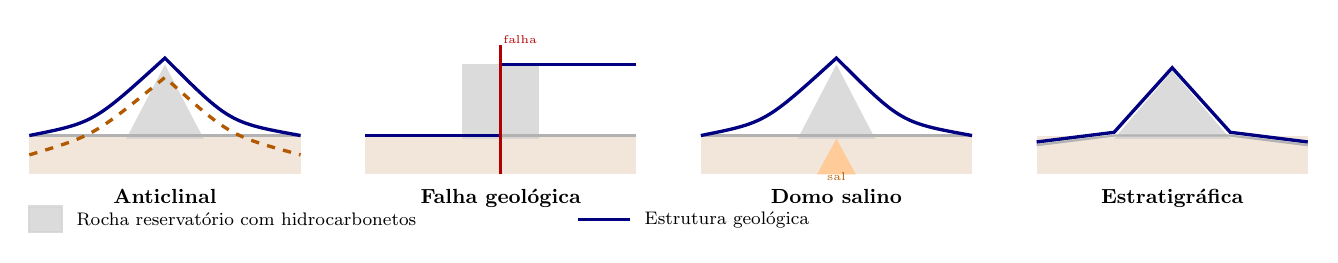
\begin{tikzpicture}[scale=0.82, transform shape, thick]
    %--- ANTICLINAL ---
    \begin{scope}[xshift=0cm]
      \fill[brown!20] (0,-0.6) rectangle (4.2,0);
      \fill[gray!35, opacity=0.8] (1.5,-0.05) -- (2.1,1.1) -- (2.7,-0.05) -- cycle;
      \draw[gray!60] (0,0) -- (4.2,0);
      \draw[blue!50!black, very thick]
        (0,0) .. controls (1,0.2) .. (2.1,1.2) .. controls (3.1,0.2) .. (4.2,0);
      \draw[orange!70!black, very thick, dashed]
        (0,-0.3) .. controls (1,0) .. (2.1,0.9) .. controls (3.1,0) .. (4.2,-0.3);
      \node[below, font=\small\bfseries] at (2.1,-0.7) {Anticlinal};
    \end{scope}
    %--- FALHA ---
    \begin{scope}[xshift=5.2cm]
      \fill[brown!20] (0,-0.6) rectangle (4.2,0);
      \fill[gray!35, opacity=0.8] (1.5,-0.05) rectangle (2.7,1.1);
      \draw[gray!60] (0,0) -- (4.2,0);
      \draw[blue!50!black, very thick] (0,0) -- (2.1,0) -- (2.1,1.1) -- (4.2,1.1);
      \draw[red!70!black, very thick] (2.1,1.4) -- (2.1,-0.6);
      \node[above, font=\tiny, red!70!black] at (2.4,1.3) {falha};
      \node[below, font=\small\bfseries] at (2.1,-0.7) {Falha geológica};
    \end{scope}
    %--- DOMO SALINO ---
    \begin{scope}[xshift=10.4cm]
      \fill[brown!20] (0,-0.6) rectangle (4.2,0);
      \fill[gray!35, opacity=0.8] (1.5,-0.05) -- (2.1,1.1) -- (2.7,-0.05) -- cycle;
      \fill[orange!40] (1.8,-0.6) -- (2.1,-0.05) -- (2.4,-0.6) -- cycle;
      \draw[gray!60] (0,0) -- (4.2,0);
      \draw[blue!50!black, very thick]
        (0,0) .. controls (1,0.2) .. (2.1,1.2) .. controls (3.1,0.2) .. (4.2,0);
      \node[below, font=\tiny, orange!70!black] at (2.1,-0.45) {sal};
      \node[below, font=\small\bfseries] at (2.1,-0.7) {Domo salino};
    \end{scope}
    %--- ESTRATIGRÁFICA ---
    \begin{scope}[xshift=15.6cm]
      \fill[brown!20] (0,-0.6) rectangle (4.2,0);
      \fill[gray!35, opacity=0.8] (1.2,-0.05) -- (2.1,1.0) -- (3.0,-0.05) -- cycle;
      \draw[gray!60] (0,-0.15) -- (1.2,0) -- (3.0,0) -- (4.2,-0.15);
      \draw[blue!50!black, very thick]
        (0,-0.1) -- (1.2,0.05) -- (2.1,1.05) -- (3.0,0.05) -- (4.2,-0.1);
      \node[below, font=\small\bfseries] at (2.1,-0.7) {Estratigráfica};
    \end{scope}
    %--- LEGENDA ---
    \draw[gray!35, fill=gray!35, opacity=0.8] (0,-1.5) rectangle (0.5,-1.1);
    \node[right, font=\footnotesize] at (0.6,-1.3) {Rocha reservatório com hidrocarbonetos};
    \draw[blue!50!black, very thick] (8.5,-1.3) -- (9.3,-1.3);
    \node[right, font=\footnotesize] at (9.4,-1.3) {Estrutura geológica};
  \end{tikzpicture}
  \caption{Principais tipos de armadilhas geológicas de petróleo: anticlinal, falha, domo salino e armadilha estratigráfica. As regiões sombreadas representam a rocha reservatório impregnada com hidrocarbonetos.}
  \label{fig:armadilhas}
  \fonte{Elaboração própria.}
\end{figure}

% -------- FOTO: Afloramento de betume / poço histórico --------
\begin{figure}[H]
  \centering
  % Substituir este fbox por \includegraphics[width=0.72\textwidth]{fotos/betume_mesopotamia.jpg}
  \fbox{\parbox{0.72\textwidth}{\centering Fotografia ou gravura histórica mostrando o uso de betume natural\\ por civilizações mesopotâmicas (c.\ 3000 a.C.).\\[4pt] \textbf{Sugestão:} ``Bitumen use in ancient Mesopotamia'' -- Wikimedia Commons (domínio público)}}
  \caption{Uso de betume natural na Mesopotâmia: a mais antiga relação documentada entre a humanidade e os hidrocarbonetos, empregado na impermeabilização de embarcações e na construção de edificações.}
  \label{fig:betume}
  \fonte{Wikimedia Commons (domínio público). [INSERIR IMAGEM REAL]}
\end{figure}

A relação humana com o petróleo, portanto, não começa com Edwin Drake
em 1859 — começa muito antes, nas margens do Eufrates, nos templos
persas e nas canoas dos povos nativos da América. O que Drake inaugurou
não foi a descoberta do petróleo, mas a sua \textit{extração
sistematizada e comercial}. E foi essa virada prática que abriu caminho
para a investigação científica que, um século e meio depois, culminou
nos enormes simuladores computacionais e nos algoritmos de aprendizado
de máquina que hoje gerenciam campos petrolíferos no fundo do Atlântico.

Em 1856, o engenheiro francês Henry Darcy formulou a lei que relaciona,
de forma quantitativa, o fluxo de fluidos a gradientes de pressão em
meios porosos \cite{dake2014, rosa2006}. Três anos mais tarde, o poço
Drake (Figura~\ref{fig:poco_drake}) provou que extrair petróleo do
subsolo era tecnicamente viável e economicamente lucrativo
\cite{yergin1991}. Esses dois marcos definem a fronteira entre a era
empírica e o nascimento da Engenharia de Reservatórios como disciplina
científica.

% -------- FOTO: Poço de Drake (Titusville, 1859) --------
\begin{figure}[H]
  \centering
  % Substituir este fbox por \includegraphics[width=0.65\textwidth]{fotos/poco_drake_1859.jpg}
  \fbox{\parbox{0.65\textwidth}{\centering Fotografia histórica do poço de Edwin L. Drake\\ em Titusville, Pensilvânia, EUA (1859).\\[4pt] \textbf{Sugestão:} ``Drake Well, Titusville Pennsylvania 1859'' -- Wikimedia Commons (domínio público, anterior a 1928)}}
  \caption{O poço Drake em Titusville, Pensilvânia (1859): o primeiro poço comercial de petróleo do mundo, com 21 metros de profundidade e produção inicial de 25 barris por dia. Este marco inaugural desencadeou a corrida global ao petróleo e transformou o mundo.}
  \label{fig:poco_drake}
  \fonte{Wikimedia Commons (domínio público). [INSERIR IMAGEM REAL]}
\end{figure}

No contexto angolano, onde o setor petrolífero representa a espinha
dorsal da economia nacional — mais de noventa por cento das exportações
e a principal fonte de receitas fiscais do país —, compreender essa
trajetória histórica não é um exercício de erudição académica. É uma
necessidade estratégica imperativa para a soberania técnica e a
segurança energética da nação.

Angola enfrenta desafios específicos nessa área: campos offshore em
águas profundas e ultra-profundas que exigem expertise em ambientes
de alta complexidade geológica; a necessidade de maximizar recuperação
de campos maduros para estender a vida produtiva do país; o imperativo
de transição para modelos de exploração mais sustentáveis; e a urgência
de desenvolver uma base técnica e científica local que não dependa
exclusivamente de expertise estrangeira.

Engenheiros capazes de gerir esses desafios — com soberania técnica,
eficiência operacional, responsabilidade socioambiental, e capacidade
de inovação — só podem ser formados se dominarem os fundamentos
históricos e teóricos sobre os quais a Engenharia de Reservatórios
foi construída. Essa formação rigorosa não apenas prepara profissionais
para operações atuais, mas também capacita Angola a liderar soluções
inovadoras em exploração sustentável de recursos energéticos, prototipagem
de tecnologias limpas (como CCS e armazenamento de hidrogénio), e
contribuição para o conhecimento global em geociências
\cite{ramos2016, ramos2020}.

% -----------------------------------------------------------
\section{Objetivos}
% -----------------------------------------------------------

\subsection{Objetivo Geral}

Investigar a evolução histórica da Engenharia de Reservatórios de
Petróleo, identificando os marcos científicos e tecnológicos
fundamentais que moldaram a disciplina desde a Antiguidade até o
século XXI, com ênfase nas implicações desse percurso para a prática
e a formação profissional em Angola.

\vspace{6pt}
\noindent
\textbf{Questão de pesquisa:} De que maneira a Engenharia de
Reservatórios de Petróleo evoluiu do empirismo artesanal para uma
disciplina quantitativa, computacional e baseada em dados, e quais são
as implicações epistemológicas e práticas desse percurso para a
formação de engenheiros de petróleo em Angola?

\subsection{Objetivos Específicos}

\begin{enumerate}[label=\alph*)]
  \item Descrever e contextualizar os antecedentes históricos da
    Engenharia de Reservatórios, com ênfase nas transições metodológicas
    e nos determinantes científicos, económicos e tecnológicos de
    cada fase;
  \item Avaliar a contribuição dos fundamentos teóricos clássicos —
    Lei de Darcy, caracterização petrofísica, análise PVT, balanço de
    materiais e análise de pressão transiente — para a consolidação da
    disciplina como ciência quantitativa;
  \item Comparar os métodos analíticos e numéricos de caracterização e
    simulação de reservatórios ao longo das diferentes fases históricas,
    evidenciando avanços, limitações e rupturas paradigmáticas;
  \item Discutir as tendências contemporâneas — Inteligência Artificial,
    Internet das Coisas, EOR e armazenamento geológico de
    CO\textsubscript{2} — e suas potenciais aplicações em contextos
    africanos e angolanos;
  \item Propor recomendações para o fortalecimento da formação e da
    investigação científica em Engenharia de Reservatórios no contexto
    angolano.
\end{enumerate}

% -----------------------------------------------------------
\section{Justificativa}
% -----------------------------------------------------------

A pertinência deste trabalho assenta em três dimensões complementares:
científica, estratégica e formativa.

Do ponto de vista \textbf{científico}, reconstruir a história de uma
disciplina é reconstruir a história do pensamento humano aplicado a um
problema concreto. No caso da Engenharia de Reservatórios, essa
reconstrução revela uma das transições mais eloquentes da história da
ciência aplicada: de práticas transmitidas por tradição oral para
algoritmos capazes de prever o comportamento de campos petrolíferos
com décadas de antecedência \cite{dake2014, rosa2006}.

Do ponto de vista \textbf{estratégico}, mesmo no cenário de transição
energética em curso, o petróleo e o gás permanecerão componentes
relevantes da matriz energética mundial por décadas. Além disso, o
conhecimento acumulado em reservatórios está sendo ativamente
reaproveitado para o armazenamento geológico de CO\textsubscript{2},
contribuindo diretamente para as metas climáticas globais
\cite{bachu2000}. A fronteira entre a engenharia de petróleo e a
engenharia climática está, pela primeira vez na história, começando
a se dissolver.

Do ponto de vista \textbf{formativo}, Angola detém reservas provadas
superiores a doze bilhões de barris e é o segundo maior produtor da
África subsaariana. Cada campo angolano que opera abaixo do seu
potencial de recuperação não é apenas uma perda económica: é um
problema de soberania técnica. A capacitação de engenheiros angolanos
com domínio sólido dos fundamentos históricos e modernos da disciplina
é, portanto, um imperativo nacional \cite{ramos2016, ramos2020}.

% -----------------------------------------------------------
\section{Metodologia}
% -----------------------------------------------------------

A presente pesquisa é de natureza bibliográfica, exploratória e
qualitativa, enquadrada no paradigma histórico-epistemológico das
ciências da engenharia. A análise foi conduzida por meio de revisão
sistemática da literatura, abrangendo publicações desde meados do
século XIX até 2026, obedecendo aos seguintes critérios de seleção:

\begin{itemize}
  \item Obras clássicas de referência internacional que estabeleceram
    os fundamentos teóricos da disciplina, incluindo as contribuições
    de Darcy (1856), Muskat (1937; 1949), Peaceman (1977) e Aziz \&
    Settari (1979);
  \item Livros-texto amplamente adotados em programas de graduação e
    pós-graduação, com cobertura abrangente dos conteúdos centrais da
    disciplina \cite{rosa2006, dake2014, mccain1990, ahmed2010,
    terry2015, alyafei2019};
  \item Obras de autoria lusófona, especialmente aquelas produzidas
    no contexto do ISPTEC \cite{ramos2016, ramos2020};
  \item Obras clássicas de referência internacional como \cite{craft1991,
    dake1994}, bem como publicações mais recentes consolidando o estado
    da arte \cite{mungan2019, spe2015};
  \item Artigos científicos seminais sobre marcos metodológicos como
    o método da derivada de pressão \cite{bourdet1989}, o balanço de
    materiais linear \cite{havlena1963} e os reservatórios não
    convencionais \cite{javadpour2009};
  \item Estudos sobre armazenamento geológico de CO\textsubscript{2}
    \cite{bachu2000};
  \item Fontes de dados sobre estatísticas energéticas e histórico industrial
    \cite{bp2023, eia2023, wikipediaReservoirEngineering, wikipediaPetroleumHistory}.
\end{itemize}

A análise foi conduzida de forma cronológica e temática, organizando
a história em quatro grandes eras que estruturam o capítulo de
Desenvolvimento.

% ============================================================
\chapter{Desenvolvimento}
\label{chap:desenvolvimento}
% ============================================================

% -----------------------------------------------------------
\section{Os Primórdios: Exploração Primitiva do Petróleo (Antiguidade ao Século XVIII)}
\label{sec:antiguidade}
% -----------------------------------------------------------

\epigraph{\textit{``Antes de ser ciência, o petróleo foi mistério,
magia e recurso prático — tudo ao mesmo tempo.''}}{--- Adaptado de
\citeonline{yergin1991}}

Imagine a surpresa de um habitante da Mesopotâmia de quatro mil anos
atrás ao perceber que certa substância escura e viscosa que brotava do
solo podia tornar um barco impermeável, fixar tijolos como nenhuma
argila conseguia e até mesmo alimentar chamas persistentes em
cerimônias religiosas. Esse material — o betume natural, primo viscoso
do petróleo — foi provavelmente a primeira forma de hidrocarboneto a
ser explorada de forma sistemática pela humanidade
\cite{yergin1991}.

As civilizações da Mesopotâmia utilizavam o betume para impermeabilizar
embarcações fluviais, assentar tijolos em grandes construções e envolver
múmias. Na Pérsia, o fogo perpétuo dos templos zoroastrianos era
alimentado por emanações naturais de gás. Os povos nativos da América
do Norte empregavam óleos de afloramento para fins medicinais e
cerimoniais. Na China, poços de bambu eram escavados já no século
IV d.C.\ para coletar salmoura e gás natural \cite{yergin1991}.

O traço comum a todas essas práticas era a completa ausência de método
sistemático: sem cálculo de volumes, sem estimativa de pressão, sem
qualquer noção do que se passava no subsolo. O ``reservatório'' era
simplesmente aquilo que brotava da terra — uma dádiva natural, não um
sistema físico a ser compreendido e gerido. O conhecimento era
transmitido por tradição oral entre gerações de artesãos, e a
``tecnologia'' se resumia a encontrar onde o óleo aflorava
espontaneamente \cite{rosa2006, ramos2016}.

Essa primeira era — da Antiguidade ao final do século XVIII —
caracteriza-se pela hegemonia do empirismo prático e pela ausência
total de fundamentação científica. Não subestime sua importância,
porém: foi precisamente essa acumulação milenar de conhecimento prático
que criou as condições culturais e económicas para a revolução
científica e industrial que viria no século seguinte.

% -----------------------------------------------------------
\section{Fundamentação Teórica: Os Séculos XIX e XX}
\label{sec:fundamentacao}
% -----------------------------------------------------------

O período entre meados do século XIX e o início do século XX
representou a mais profunda transformação epistemológica da história
da Engenharia de Reservatórios: a passagem do ofício artesanal para a
disciplina científica rigorosa. Dois desenvolvimentos paralelos
impulsionaram essa transição. Por um lado, o estabelecimento de
fundamentos teóricos sólidos, ancorados na física do escoamento em
meios porosos. Por outro, o início da exploração comercial sistemática,
que gerou a demanda económica necessária para financiar a investigação
científica \cite{dake2014, rosa2006}.

% - - - - - - - - - - - - - - - - - - - - - - - - - - - - - -
\subsection{Henry Darcy e a Lei Fundamental do Escoamento em Meios Porosos}
% - - - - - - - - - - - - - - - - - - - - - - - - - - - - - -

Há algo profundamente belo no fato de que a lei mais fundamental da
Engenharia de Reservatórios não tenha sido derivada por um engenheiro
de petróleo — ela sequer existia como disciplina na época —, mas por
um engenheiro sanitário francês preocupado com o abastecimento de água
da cidade de Dijon. Essa é a história de \textbf{Henry Philibert
Gaspard Darcy} (1803--1858), e ela diz muito sobre como a ciência
realmente funciona: as grandes descobertas raramente chegam de onde
esperamos.

% -------- FOTO/RETRATO: Henry Darcy --------
\begin{figure}[H]
  \centering
  % Substituir este fbox por \includegraphics[width=0.40\textwidth]{fotos/henry_darcy_retrato.jpg}
  \fbox{\parbox{0.40\textwidth}{\centering Retrato de Henry Philibert Gaspard Darcy\\ (Dijon, França, 1803--1858), engenheiro hidráulico\\ cujos experimentos com colunas de areia deram origem\\ à lei fundamental da Engenharia de Reservatórios.\\[4pt] \textbf{Sugestão:} ``Henri Darcy'' -- Wikimedia Commons (domínio público)}}
  \caption{Henry Darcy (1803--1858): engenheiro hidráulico francês que, ao estudar o sistema de abastecimento de água de Dijon, formulou em 1856 a lei fundamental do escoamento de fluidos em meios porosos — o alicerce matemático de toda a Engenharia de Reservatórios moderna.}
  \label{fig:darcy_retrato}
  \fonte{Wikimedia Commons (domínio público). [INSERIR IMAGEM REAL]}
\end{figure}

Ao estudar o sistema de abastecimento de água de Dijon, Darcy realizou
experimentos sistemáticos com colunas de areia e formulou, em 1856,
a lei que rege o escoamento de fluidos newtonianos em meios porosos
sob regime permanente \cite{dake2014, rosa2006}. A
\textbf{Lei de Darcy}, expressa pela Equação~\ref{eq:darcy},
estabelece uma relação de proporcionalidade entre a vazão volumétrica
do fluido e o gradiente de pressão, mediada pelas propriedades do meio
(permeabilidade) e do fluido (viscosidade):

\begin{equation}
  q = -\frac{kA}{\mu}\frac{dP}{dL}
  \label{eq:darcy}
\end{equation}

\noindent onde $q$ é a vazão volumétrica (cm\textsuperscript{3}/s),
$k$ é a permeabilidade absoluta do meio (Darcy), $A$ é a área da
seção transversal (cm\textsuperscript{2}), $\mu$ é a viscosidade
dinâmica do fluido (cP) e $dP/dL$ é o gradiente de pressão
(atm/cm). O sinal negativo indica que o escoamento se dá no sentido
do declínio de pressão \cite{rosa2006}.

A importância dessa equação não pode ser superestimada. Ela tornou
possível a estimativa quantitativa de vazão e produtividade de poços,
constituindo o ponto de partida para toda a teoria moderna de
escoamento em reservatórios. Ao longo do século XX, a Lei de Darcy
foi generalizada para escoamentos multifásicos, para geometrias
radiais e esféricas, e integrada com as equações de conservação de
massa para originar as equações diferenciais parciais que governam
os simuladores numéricos de reservatórios \cite{alyafei2019, rosa2006}.

% - - - - - - - - - - - - - - - - - - - - - - - - - - - - - -
\subsection{O Início da Indústria Petrolífera Moderna}
% - - - - - - - - - - - - - - - - - - - - - - - - - - - - - -

No dia 27 de agosto de 1859, um antigo condutor de trem chamado
\textbf{Edwin Laurentine Drake} perfurou um poço de 21 metros de
profundidade em Titusville, Pensilvânia, e mudou o mundo. A produção
inicial era modesta — cerca de 25 barris por dia —, mas o que Drake
provou era muito maior do que essa quantidade sugeria: o petróleo
podia ser extraído de forma \textit{controlada, repetível e
economicamente viável} mediante perfuração \cite{yergin1991}.

O que se seguiu foi uma corrida global ao ``ouro negro'' sem
precedentes na história industrial. Em pouco tempo, campos foram
descobertos na Rússia (Baku, 1870), na Indonésia (1880), no México
e no Oriente Médio (1908, com o campo de Masjid-i-Suleiman, no atual
Irã). Mas apesar do crescimento exponencial da produção, a extração
ainda era conduzida de forma essencialmente empírica. Não existiam
métodos para estimar o volume de óleo \textit{in situ}, prever
a curva de declínio de produção ou identificar os mecanismos de
expulsão do óleo. Os campos eram frequentemente abandonados com
recuperações de apenas dez a quinze por cento do OOIP, simplesmente
porque ninguém compreendia o que se passava no subsolo
\cite{terry2015}.

% -------- FOTO: Campo petrolífero histórico (Baku / Pensilvânia) --------
\begin{figure}[H]
  \centering
  % Substituir este fbox por \includegraphics[width=0.80\textwidth]{fotos/campo_petrolifero_1890.jpg}
  \fbox{\parbox{0.80\textwidth}{\centering Fotografia histórica de campo petrolífero do final do século XIX\\ (Baku, Azerbaijão, c.\ 1890, ou Pensilvânia, EUA, c.\ 1865).\\ As torres de madeira (derricks) eram perfuradas sem qualquer\\ modelo de subsolo, puramente pelo método de tentativa e erro.\\[4pt] \textbf{Sugestão:} ``Baku oil fields 1890'' ou ``Oil Creek Pennsylvania 1865'' -- Wikimedia Commons (domínio público)}}
  \caption{Campo petrolífero do final do século XIX: a floresta de torres de perfuração simboliza o ritmo febril de exploração do período, conduzida sem qualquer modelo geológico ou reservatório, com taxas de recuperação frequentemente inferiores a 15\% do OOIP.}
  \label{fig:campo_historico}
  \fonte{Wikimedia Commons (domínio público). [INSERIR IMAGEM REAL]}
\end{figure}

% -----------------------------------------------------------
\section{Propriedades Fundamentais de Rocha e Fluido}
\label{sec:propriedades}
% -----------------------------------------------------------

Para construir qualquer modelo de reservatório — por mais simples que
seja —, é preciso saber duas coisas fundamentais sobre a rocha: quanto
espaço ela tem disponível para armazenar fluidos, e com que facilidade
esses fluidos conseguem se mover dentro dela. Essas duas perguntas,
aparentemente simples, deram origem a décadas de investigação
laboratorial e de campo que constituem a base da petrofísica
\cite{rosa2006, mccain1990}.

% - - - - - - - - - - - - - - - - - - - - - - - - - - - - - -
\subsection{Porosidade e Permeabilidade}
% - - - - - - - - - - - - - - - - - - - - - - - - - - - - - -

A \textbf{porosidade} ($\phi$) é a fração do volume total da rocha
ocupada por espaços vazios:

\begin{equation}
  \phi = \frac{V_p}{V_t} = \frac{V_t - V_s}{V_t}
  \label{eq:poro}
\end{equation}

A distinção entre \textit{porosidade total} e \textit{porosidade
efetiva} — o espaço poral interconectado, acessível ao fluido — foi
um refinamento conceitual fundamental desenvolvido nas décadas de 1920
e 1930. Uma rocha pode ser muito porosa e ainda assim improdutiva, se
os seus poros não estiverem conectados entre si \cite{alyafei2019}.

A \textbf{permeabilidade} quantifica a facilidade com que fluidos
atravessam o meio poroso sob a ação de um gradiente de pressão.
Expressa em Darcy ou em milidarcy (mD), ela é uma propriedade
intrinsecamente ligada à geometria do espaço poral — tamanho, formato
e conectividade dos poros. Reservatórios convencionais apresentam
permeabilidades típicas entre 1\,mD e alguns Darcies; reservatórios
de \textit{shale} podem apresentar valores inferiores a 0{,}001\,mD
\cite{javadpour2009}.

% -------- FOTO: Imagem de microscopia de plugue de testemunho --------
\begin{figure}[H]
  \centering
  % Substituir este fbox por \includegraphics[width=0.70\textwidth]{fotos/microscopio_rocha_reservatorio.jpg}
  \fbox{\parbox{0.70\textwidth}{\centering Imagem de Microscopia Eletrônica de Varredura (MEV)\\ de arenito ou carbonato, mostrando a estrutura dos poros\\ e a geometria do espaço poral que controla porosidade\\ e permeabilidade da rocha reservatório.\\[4pt] \textbf{Sugestão:} ``Sandstone SEM pore structure'' -- MDPI Open Access ou Wikimedia Commons}}
  \caption{Imagem de microscopia de rocha reservatório: a estrutura microscópica dos poros controla diretamente as propriedades petrofísicas (porosidade e permeabilidade) que determinam a capacidade produtiva do reservatório.}
  \label{fig:microscopio_rocha}
  \fonte{[INSERIR REFERÊNCIA DA IMAGEM REAL]}
\end{figure}

O conceito de \textbf{permeabilidade relativa}, formulado por Leverett
e Lewis (1941), descreve o comportamento de cada fase fluida (óleo,
água e gás) quando duas ou mais fases coexistem nos poros. As curvas
de permeabilidade relativa são dependentes da saturação de cada fase
e da história de molhabilidade da rocha, sendo indispensáveis para
a modelagem do deslocamento multifásico \cite{rosa2006}.

% - - - - - - - - - - - - - - - - - - - - - - - - - - - - - -
\subsection{Análise PVT e Classificação dos Fluidos de Reservatório}
% - - - - - - - - - - - - - - - - - - - - - - - - - - - - - -

% FIGURA 4 – Diagrama PVT (TikZ)
\begin{figure}[H]
  \centering
  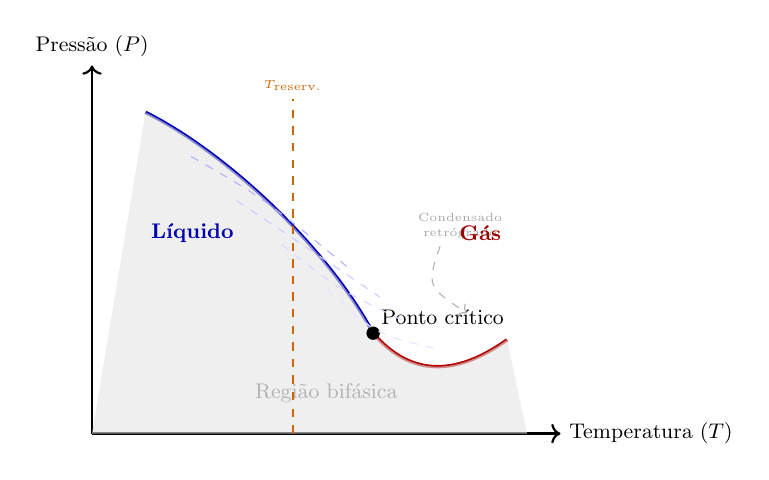
\begin{tikzpicture}[scale=0.85, transform shape]
    \draw[->, thick] (0,0) -- (7,0) node[right] {\small Temperatura ($T$)};
    \draw[->, thick] (0,0) -- (0,5.5) node[above] {\small Pressão ($P$)};
    % Curva de bolha (bubble point)
    \draw[blue!70!black, very thick]
      (0.8,4.8) .. controls (2,4.2) and (3.5,2.8) .. (4.2,1.5);
    % Curva de orvalho (dew point)
    \draw[red!70!black, very thick]
      (4.2,1.5) .. controls (4.8,0.8) and (5.5,0.9) .. (6.2,1.4);
    % Região bifásica
    \fill[gray!20, opacity=0.6]
      (0.8,4.8) .. controls (2,4.2) and (3.5,2.8) .. (4.2,1.5)
                .. controls (4.8,0.8) and (5.5,0.9) .. (6.2,1.4)
                -- (6.5,0) -- (0,0) -- cycle;
    % Ponto crítico
    \fill[black] (4.2,1.5) circle (0.1);
    \node[above right, font=\small] at (4.2,1.5) {Ponto crítico};
    % Linhas de qualidade (isovolumes)
    \foreach \frac/\col in {0.2/blue!30,0.4/blue!20,0.6/blue!15,0.8/blue!10}
      \draw[\col, thin, dashed]
        ($(0.8,4.8)!\frac!(4.2,1.5)$) .. controls
        ($(2,4.2)!\frac!(4.8,0.8)$) ..
        ($(3.5,2.8)!\frac!(5.5,0.9)$);
    % Seta condensado retrógrado
    \draw[->, dashed, gray!60]
      (5.2,2.8) .. controls (5.0,2.2) .. (5.6,1.8);
    \node[font=\tiny, gray!70, align=center] at (5.5,3.1)
      {Condensado\\retrógrado};
    % Labels de regiões
    \node[font=\small\bfseries, blue!70!black] at (1.5,3.0) {Líquido};
    \node[font=\small\bfseries, red!60!black] at (5.8,3.0) {Gás};
    \node[font=\small, gray!60] at (3.5,0.6) {Região bifásica};
    % Linha isoterma de reservatório (exemplo) - CORREÇÃO: \rm -> \textnormal
    \draw[orange!80!black, thick, dashed] (3.0,0) -- (3.0,5.0);
    \node[above, font=\tiny, orange!80!black] at (3.0,5.0) {$T_{\textnormal{reserv.}}$};
  \end{tikzpicture}
  \caption{Diagrama de fases PVT esquemático, ilustrando a envoltória de fases, o ponto crítico e a região de condensado retrógrado. A posição da temperatura de reservatório em relação à envoltória determina o tipo de fluido e a estratégia de produção adequada.}
  \label{fig:pvt}
  \fonte{Adaptado de \citeonline{mccain1990}.}
\end{figure}

As propriedades dos fluidos de reservatório variam significativamente
com a pressão e a temperatura, e devem ser determinadas por análises
PVT. A obra de \cite{mccain1990} consolidou-se como a referência
definitiva para correlação e predição dessas propriedades, reunindo
décadas de dados experimentais de campos ao redor do mundo.

Com base no diagrama PVT (Figura~\ref{fig:pvt}), os fluidos foram
classificados em cinco categorias \cite{mccain1990, ahmed2010}:
\textit{óleo negro}, \textit{óleo volátil}, \textit{gás condensado
retrógrado}, \textit{gás úmido} e \textit{gás seco}. Cada categoria
exige uma estratégia de desenvolvimento e instalações de superfície
específicas, tornando a caracterização PVT um passo anterior e
obrigatório a qualquer plano de desenvolvimento de campo.

% -----------------------------------------------------------
\section{Consolidação Científica: O Século XX}
\label{sec:seculo_xx}
% -----------------------------------------------------------

O século XX é, sem exagero, a era de ouro da Engenharia de
Reservatórios. As duas guerras mundiais e a industrialização acelerada
criaram uma demanda energética sem precedentes, e o petróleo estava
no centro de tudo: movia tanques, aviões, navios e fábricas. Essa
pressão — económica, política e estratégica — comprimiu décadas de
desenvolvimento científico normal em poucos anos e transformou a
engenharia de reservatórios de uma prática artesanal em uma ciência
rigorosa \cite{muskat1949, peaceman1977}.

% - - - - - - - - - - - - - - - - - - - - - - - - - - - - - -
\subsection{Muskat e a Sistematização da Engenharia de Reservatórios}
% - - - - - - - - - - - - - - - - - - - - - - - - - - - - - -

Se Darcy deu à disciplina a sua equação fundamental, \textbf{Morris
Muskat} (1900--1998) deu-lhe a sua estrutura teórica completa. Com
formação em física teórica e uma capacidade analítica extraordinária,
Muskat abordou os problemas de reservatórios com o rigor matemático
de um físico e a sensibilidade prática de um engenheiro de campo.

Em \textit{The Flow of Homogeneous Fluids Through Porous Media} (1937)
e em \textit{Physical Principles of Oil Production} (1949), Muskat
integrou a Lei de Darcy com as equações de continuidade e de estado
dos fluidos, estabelecendo as bases matemáticas dos mecanismos de
produção e da recuperação secundária \cite{muskat1949}. Nessas obras,
o engenheiro deixou de ser um empirista que ``sabia o que funcionava''
e passou a ser um cientista capaz de \textit{prever} o comportamento
de um reservatório antes de perfurar um único poço novo.

% - - - - - - - - - - - - - - - - - - - - - - - - - - - - - -
\subsection{Mecanismos de Produção de Reservatórios}
% - - - - - - - - - - - - - - - - - - - - - - - - - - - - - -

Uma das contribuições mais práticas do século XX foi a identificação
sistemática dos mecanismos naturais que impulsionam os fluidos do
reservatório em direção ao poço. Compreender esses mecanismos é
compreender a energia que o próprio reservatório carrega — e como
aproveitá-la de forma inteligente \cite{terry2015}.

Os cinco mecanismos primários identificados são:

\begin{enumerate}[label=\roman*.]
  \item \textbf{Expansão de fluido e rocha}: a energia armazenada sob
    a forma de compressibilidade do óleo, da água connata e da rocha
    é liberada à medida que a pressão declina. É o mecanismo mais
    simples — e também o menos eficiente em termos de recuperação;
  \item \textbf{Gás em solução} (\textit{solution gas drive}): abaixo
    da pressão de bolha, o gás dissolvido se liberta e expande,
    empurrando o óleo em direção ao poço. A eficiência deteriora-se
    quando a saturação de gás livre supera o valor crítico, pois
    o gás começa a fluir preferencialmente;
  \item \textbf{Capa de gás} (\textit{gas cap drive}): a expansão de
    uma capa de gás livre no topo do reservatório auxilia na expulsão
    do óleo, com eficiência superior ao gás em solução;
  \item \textbf{Influxo de água} (\textit{water drive}): a expansão
    do aquífero associado desloca o óleo para os poços — tipicamente
    o mecanismo de maior fator de recuperação, podendo atingir 50 a
    70\% do OOIP;
  \item \textbf{Segregação gravitacional}: a diferença de densidades
    entre gás, óleo e água induz separação vertical natural, que pode
    ser aproveitada em estratégias de \textit{gravity drainage}.
\end{enumerate}

Na prática, a maioria dos reservatórios opera sob influência combinada
de dois ou mais mecanismos, e identificar o mecanismo dominante é
decisivo para a estratégia de recuperação secundária
\cite{rosa2006, ahmed2010}.

% - - - - - - - - - - - - - - - - - - - - - - - - - - - - - -
\subsection{Evolução dos Métodos de Recuperação de Petróleo}
% - - - - - - - - - - - - - - - - - - - - - - - - - - - - - -

A recuperação de petróleo refere-se ao conjunto de técnicas utilizadas
para extrair hidrocarbonetos dos reservatórios subterrâneos de forma
economicamente viável. Historicamente, a evolução desses métodos
acompanha precisamente a evolução da compreensão teórica dos
mecanismos de produção: começou-se com aproveitamento passivo da
energia natural e caminhou-se progressivamente para técnicas sofisticadas
de deslocamento artificial \cite{ahmed2010, terry2015, rosa2006}.

\subsubsection{Recuperação Primária}

A \textbf{recuperação primária} utiliza exclusivamente a energia
natural do reservatório para deslocar o petróleo até os poços. Durante
essa fase, apenas um ou mais dos mecanismos naturais descritos
anteriormente — expansão de fluido, gás dissolvido, pressão de influxo
de água ou segregação gravitacional — atuam para expulsar o óleo.

Na era inicial da indústria (século XIX até meados do século XX), a
recuperação primária era a única técnica disponível. Os campos eram
frequentemente explorados sob essa modalidade até que a pressão
decaísse a ponto de tornar a produção economicamente inviável. O fator
de recuperação tipicamente não ultrapassava 15\%, em alguns casos
inferiores a 10\% do \textit{Original Oil In Place} (OOIP). Essa
ineficiência era aceita como inevitável — uma consequência da física
e da tecnologia da época, não uma deficiência de planejamento
\cite{terry2015, rosa2006}.

\subsubsection{Recuperação Secundária}

A \textbf{recuperação secundária} surgiu a partir da década de 1930,
com a realização de que pressão de reservatório prorrogada artificialmente
poderia recuperar quantidades significativamente maiores de óleo. Os
dois principais métodos são:

\begin{itemize}
  \item \textbf{Injeção de água}: fluido injetado em poços periféricos
    ou estrategicamente localizados expande o aquífero associado ou
    introduce um novo banco de deslocamento. A água também é a opção
    mais económica em operações de grande escala. Tornou-se amplamente
    utilizada a partir das décadas de 1940 e 1950;
  \item \textbf{Injeção de gás}: gás natural separado da produção é
    recomprimido e reinjetado para manter a pressão. Oferece a vantagem
    de aproveitar o gás que seria queimado (\textit{flared}) ou descartado,
    embora seja menos eficiente que a injeção de água em termos de
    varrimento.
\end{itemize}

A adoção sistemática da injeção de água aumentou drasticamente os
fatores de recuperação dos reservatórios explorados até então. Campos
que haviam sido abandonados com recuperações de 20 a 30\% do OOIP
puderam ser reexplorados com as novas técnicas, elevando a recuperação
final para 50\% ou mais em casos favoráveis. Esse aumento não era
trivial: representava receita e vida útil estendidas de várias décadas \cite{ahmed2010}.

\subsubsection{Da Recuperação Secundária para a Avançada (EOR)}

Mesmo com a injeção de água ou gás bem executada, uma fração significativa
de óleo permanecia imobilizada nos poros. Nos campos maduros do final
do século XX, era comum encontrar 50 a 70\% do OOIP ainda \textit{in
situ} após as fases primária e secundária. Essa constatação abriu caminho
para a investigação de método mais agressivos — as técnicas de
\textbf{Recuperação Avançada de Petróleo (EOR)}, que visam alterar
as propriedades físicas ou químicas dos fluidos ou do reservatório
para mobilizar óleo residual \cite{lake2007}.

As técnicas EOR podem ser classificadas segundo diversos critérios. A
mais simples categorização agrupa-as em térmicas, miscíveis, químicas
e microbiológicas — cada uma operando segundo mecanismos distintos,
adequadas a tipos específicos de óleo e rocha, e exigindo análise
económica cuidadosa \cite{ahmed2010, terry2015}.

Os métodos térmicos (principalmente injeção de vapor ou combustão no
local) aquecem o óleo in situ, reduzindo significativamente a sua
viscosidade e melhorando a mobilidade em reservatórios com óleos pesados.
Os métodos miscíveis (injeção de gases como CO\textsubscript{2} ou
hidrocarbonetos leves) estabelecem miscibilidade com o óleo, eliminando
a tensão interfacial e permitindo mobilização do fluido residual. Os
métodos químicos (polímeros, surfactantes, soluções alcalinas) modificam
as propriedades do deslocamento ou reduzem a adsorção de óleo às
superfícies de rocha, aumentando a razão de mobilidade favorável.
Independentemente do método escolhido, o sucesso de qualquer projeto EOR
depende de análise rigorosa da compatibilidade rocha-fluido, estimativa
precisa de custos e receitas, e monitoramento contínuo do desempenho
durante a operação.

% - - - - - - - - - - - - - - - - - - - - - - - - - - - - - -
\subsection{O Método do Balanço de Materiais}
% - - - - - - - - - - - - - - - - - - - - - - - - - - - - - -

Há uma elegância genuína no método do balanço de materiais: a ideia de
que é possível ``pesar'' um reservatório — estimar o seu volume
original de óleo e identificar os seus mecanismos de produção — usando
apenas os dados históricos de pressão e produção, sem abrir um único
metro quadrado de rocha. Trata-se de um dos resultados mais poderosos
e duradouros de toda a disciplina \cite{ahmed2010, rosa2006}.

Fundamentado no princípio de conservação de massa, a equação geral
do balanço de materiais para um reservatório de óleo com capa de gás
e aquífero é \cite{rosa2006}:

\begin{equation}
\begin{split}
& N_p\left[B_o + (R_p - R_s)B_g\right] + W_p B_w = \\
& N\left[(B_o - B_{oi}) + m B_{oi}\!\left(\frac{B_g}{B_{gi}}-1\right)
+ (1+m)B_{oi}\frac{c_w S_{wi}+c_f}{1-S_{wi}}\Delta P\right]
+ W_e B_w
\label{eq:balance}
\end{split}
\end{equation}

O lado esquerdo representa o volume total de fluidos produzidos; o
lado direito, as fontes de energia que os expulsaram. A reformulação
gráfica de \cite{havlena1963} simplificou enormemente a aplicação
prática: ao representar a equação como uma relação linear entre
funções dos dados de produção e pressão, os autores tornaram possível
a identificação \textit{gráfica} dos mecanismos dominantes e o
diagnóstico de inconsistências nos dados — uma abordagem que ainda
hoje é indispensável para verificação de modelos de simulação
\cite{rosa2006, dake2014}.

% - - - - - - - - - - - - - - - - - - - - - - - - - - - - - -
\subsection{Análise de Pressão Transiente}
% - - - - - - - - - - - - - - - - - - - - - - - - - - - - - -

Imagine poder ``enxergar'' dentro de um reservatório a centenas de
metros de profundidade, identificar falhas geológicas, zonas de alta
permeabilidade e limites estruturais — usando apenas dados de pressão
medidos em superfície. É exatamente isso que a análise de pressão
transiente permite fazer \cite{dake2014}.

O método de \textit{buildup} de Horner (1951) foi pioneiro ao permitir
a estimativa de permeabilidade e de \textit{skin} a partir de curvas
logarítmicas de restauração de pressão. A revolução definitiva nessa
área veio em 1983 com a introdução do \textbf{método da derivada de
pressão} por \cite{bourdet1989}: a análise da derivada revelou
características do reservatório — falhas, zonas de alta permeabilidade,
limites externos, dupla porosidade — que eram invisíveis nas curvas
convencionais. Esse avanço transformou definitivamente a análise de
pressão em uma técnica de diagnóstico de reservatórios de precisão
cirúrgica \cite{dake2014}.

% - - - - - - - - - - - - - - - - - - - - - - - - - - - - - -
\subsection{Estimativa de Volumes e Reservas: Evolução Metodológica}
% - - - - - - - - - - - - - - - - - - - - - - - - - - - - - -

Paralelamente ao desenvolvimento de métodos de análise de comportamento
dinâmico (balanço de materiais, análise de pressão), a engenharia de
reservatórios também evoluiu na estimativa prospectiva do volume original
de hidrocarbonetos. Essa quantificação é crítica: decisões bilionárias
de desenvolvimento de campos baseiam-se em estimativas de volume, e uma
incerteza de $\pm 50\%$ pode transformar um projeto viável em
antieconômico \cite{rosa2006}.

A evolução dos métodos de estimativa de volumes reflete a progressão
geral da disciplina de empirismo para rigor científico:

\paragraph{1. Método da Analogia.}
Empregado antes da perfuração do poço descobridor, este método utiliza
dados detalhados de reservatórios similares geologicamente para estimar
volumes probáveis do novo campo. Embora intuitivo, o método sofre com a
incerteza intrínseca: campos geologicamente similares podem apresentar
volumes radicalmente diferentes devido a variações em porosidade ou
tamanho \cite{rosa2006}.

\paragraph{2. Análise de Risco Probabilística.}
Aplica tratamento estatístico robusto aos parâmetros incertos (porosidade,
saturação, fator volume de formação) gerando distribuições de
probabilidade para volumes de reservas. Tipicamente, produz estimativas
pessimista (P90), provável (P50) e otimista (P10), quantificando
rigorosamente a incerteza associada a cada parâmetro \cite{ahmed2010}.

\paragraph{3. Método Volumétrico Integrado.}
Integra mapeamento geológico de alta resolução com dados de poços e
sísmica para calcular volume original através da equação clássica:
$V_o = A \times h \times \phi \times (1-S_w)$, onde $A$ é a área, $h$
a espessura, $\phi$ a porosidade, $S_w$ a saturação inicial de água.
Este é o método padrão da indústria para campos explorados, oferecendo
precisão quando a cobertura petrofísica e geológica é adequada \cite{rosa2006}.

\paragraph{4. Método de Performance/Declínio.}
Empregado retrospectivamente, utiliza histórico de produção, dados de
balanço de materiais e simulação numérica para confirmar ou ajustar
estimativas de volume após anos de operação. Oferece validação prática,
mas apenas quando suficientes dados dinâmicos acumularam-se \cite{ahmed2010}.

Na prática moderna, combinam-se múltiplos métodos para reduzir incerteza
e criar estimativas robustas de volume recuperável, base fundamental
para a estratégia econômica de desenvolvimento de campos.

% - - - - - - - - - - - - - - - - - - - - - - - - - - - - - -
\subsection{A Modelagem Computacional como Ruptura Paradigmática}
% - - - - - - - - - - - - - - - - - - - - - - - - - - - - - -

Na segunda metade do século XX, a chegada do computador digital mudou
as regras do jogo para sempre. De repente, era possível resolver
sistemas de equações diferenciais parciais em geometrias
tridimensionais com propriedades variáveis — algo absolutamente
inviável para um ser humano com papel e caneta. A simulação
computacional de reservatórios havia chegado \cite{aziz1979, peaceman1977}.

% FIGURA 5 – Malha de simulação (TikZ melhorado)
\begin{figure}[H]
  \centering
  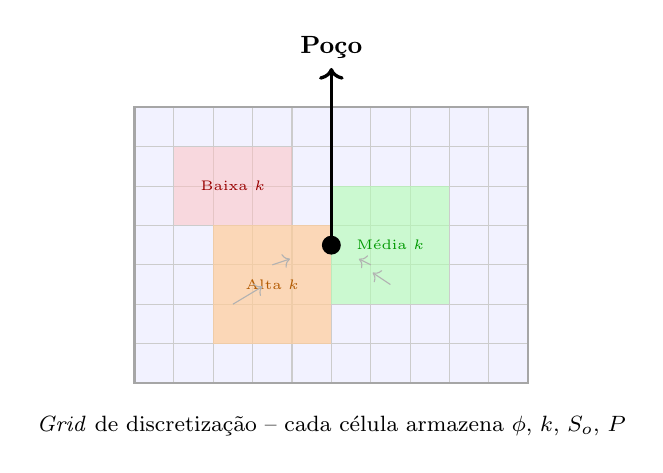
\begin{tikzpicture}[scale=1.0]
    % Plano de fundo da grade
    \fill[blue!5] (0,0) rectangle (5,3.5);
    % Grade principal
    \draw[step=0.5, gray!40, thin] (0,0) grid (5,3.5);
    \draw[thick, gray!70] (0,0) rectangle (5,3.5);
    % Células com diferentes permeabilidades (heterogeneidade)
    \fill[orange!40, opacity=0.7] (1.0,0.5) rectangle (2.5,2.0);
    \fill[green!30, opacity=0.6] (2.5,1.0) rectangle (4.0,2.5);
    \fill[red!25, opacity=0.5] (0.5,2.0) rectangle (2.0,3.0);
    % Poço produtor
    \fill[black] (2.5,1.75) circle (0.12);
    \draw[->, very thick, black] (2.5,1.75) -- (2.5,4.0);
    \node[above, font=\small\bfseries] at (2.5,4.0) {Poço};
    % Legenda de permeabilidade
    \node[font=\tiny, orange!70!black] at (1.75,1.25) {Alta $k$};
    \node[font=\tiny, green!60!black] at (3.25,1.75) {Média $k$};
    \node[font=\tiny, red!60!black] at (1.25,2.5) {Baixa $k$};
    % Setas de fluxo
    \foreach \x/\y in {1.25/1.0, 1.75/1.5, 3.0/1.5, 3.25/1.25}
      \draw[->, gray!60, thin] (\x,\y) -- ($(2.5,1.75)!0.7!(\x,\y)$);
    \node[below, font=\footnotesize] at (2.5,-0.3) {\textit{Grid} de discretização -- cada célula armazena $\phi$, $k$, $S_o$, $P$};
  \end{tikzpicture}
  \caption{Representação de uma malha de simulação numérica com heterogeneidade de permeabilidade. Cada célula armazena valores de porosidade, permeabilidade, saturação e pressão, constituindo a unidade computacional básica do simulador. A diversidade de cores ilustra a variação espacial de permeabilidade — a realidade de qualquer campo real.}
  \label{fig:grid}
  \fonte{Elaboração própria.}
\end{figure}

A equação de difusividade — base dos primeiros simuladores, derivada
da combinação da Lei de Darcy com a equação de continuidade —
é \cite{rosa2006}:

\begin{equation}
  \nabla^2 P = \frac{\phi \mu c_t}{k}\frac{\partial P}{\partial t}
  \label{eq:difusividade}
\end{equation}

A obra fundamental de \cite{peaceman1977} estabeleceu os métodos
numéricos de discretização por diferenças finitas; \cite{aziz1979}
sistematizou os métodos de volumes finitos para geometrias mais
complexas. As primeiras versões comerciais de simuladores surgiram nos
anos 1970--1980, e sua difusão representou uma mudança definitiva na
prática profissional: o engenheiro de reservatórios ganhou, pela
primeira vez, a capacidade de prever o futuro de um campo com décadas
de antecedência.

% -------- FOTO: Simulador de reservatório moderno (interface de software) --------
\begin{figure}[H]
  \centering
  % Substituir este fbox por \includegraphics[width=0.80\textwidth]{fotos/simulador_reservatorio.png}
  \fbox{\parbox{0.80\textwidth}{\centering Interface de software de simulação numérica de reservatórios\\ (ex.: Eclipse, CMG IMEX, tNavigator ou Petrel RE),\\ mostrando modelo 3D de um campo com distribuição\\ de saturação de óleo após simulação.\\[4pt] \textbf{Sugestão:} material educacional do fabricante (SLB/Schlumberger,\\ CMG, Rock Flow Dynamics) -- verificar licença de uso.}}
  \caption{Interface de simulação numérica de reservatório moderno: o modelo tridimensional permite visualizar a distribuição de saturação, pressão e fluxo em um campo inteiro, integrando dados geológicos, petrofísicos e de produção em uma única plataforma de análise.}
  \label{fig:simulador}
  \fonte{[INSERIR REFERÊNCIA DO SOFTWARE / IMAGEM REAL]}
\end{figure}

% -----------------------------------------------------------
\section{A Era Digital e os Desafios Contemporâneos}
\label{sec:digital}
% -----------------------------------------------------------

\epigraph{\textit{``O maior reservatório do século XXI não é de petróleo
— é de dados. E quem souber refiná-los terá a maior vantagem
competitiva da história.''}}{--- Paráfrase de perspectiva da
indústria 4.0}

O início do século XXI introduziu um novo paradigma para a Engenharia
de Reservatórios, caracterizado pela convergência entre modelagem
física clássica, monitoramento em tempo real por sensores digitais e
técnicas de aprendizado de máquina. Essa convergência não apenas
aumenta a precisão das análises — ela transforma a natureza do trabalho
do engenheiro, que deixa de ser um analista de dados históricos e passa
a operar em um ambiente de decisão contínua e orientada por dados em
tempo real \cite{ramos2020, ahmed2010}.

% - - - - - - - - - - - - - - - - - - - - - - - - - - - - - -
\subsection{Recuperação Avançada de Petróleo (EOR)}
% - - - - - - - - - - - - - - - - - - - - - - - - - - - - - -

% FIGURA 6 – Métodos EOR (TikZ melhorado)
\begin{figure}[H]
  \centering
  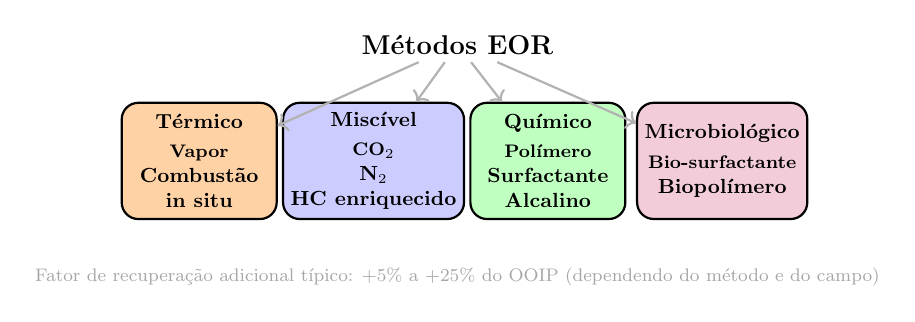
\begin{tikzpicture}[scale=0.82, transform shape, node distance=0.8cm]
    % Título central
    \node[font=\large\bfseries, align=center] (titulo) at (5.5,4.0) {Métodos EOR};
    % Caixas de métodos
    \node[draw, rounded corners=6pt, fill=orange!35, thick,
          minimum width=2.4cm, minimum height=1.8cm,
          font=\small\bfseries, align=center] (termico) at (1.5,2.2)
          {Térmico\\[2pt]\footnotesize Vapor\\Combustão\\in situ};
    \node[draw, rounded corners=6pt, fill=blue!20, thick,
          minimum width=2.4cm, minimum height=1.8cm,
          font=\small\bfseries, align=center] (miscivel) at (4.2,2.2)
          {Miscível\\[2pt]\footnotesize CO$_2$\\N$_2$\\HC enriquecido};
    \node[draw, rounded corners=6pt, fill=green!25, thick,
          minimum width=2.4cm, minimum height=1.8cm,
          font=\small\bfseries, align=center] (quimico) at (6.9,2.2)
          {Químico\\[2pt]\footnotesize Polímero\\Surfactante\\Alcalino};
    \node[draw, rounded corners=6pt, fill=purple!20, thick,
          minimum width=2.4cm, minimum height=1.8cm,
          font=\small\bfseries, align=center] (micro) at (9.6,2.2)
          {Microbiológico\\[2pt]\footnotesize Bio-surfactante\\Biopolímero};
    % Setas do título para caixas
    \foreach \node in {termico, miscivel, quimico, micro}
      \draw[->, thick, gray!60] (titulo) -- (\node);
    % Fator de recuperação típico
    \node[font=\footnotesize, gray!70, align=center] at (5.5,0.4)
      {Fator de recuperação adicional típico: +5\% a +25\% do OOIP (dependendo do método e do campo)};
  \end{tikzpicture}
  \caption{Categorias de métodos de Recuperação Avançada de Petróleo (EOR). A seleção do método adequado depende das propriedades do fluido e da rocha, das condições de pressão e temperatura do reservatório, e da análise económica do campo.}
  \label{fig:eor}
  \fonte{Adaptado de \citeonline{ahmed2010}.}
\end{figure}

Em campos maduros, a fração de óleo não recuperada pode superar 60\%
do OOIP — um enorme potencial économico e estratégico à espera de
tecnologia adequada. Os métodos EOR visam mobilizar esse óleo residual
mediante a alteração das propriedades dos fluidos ou do escoamento no
reservatório \cite{ahmed2010, terry2015}:

\begin{itemize}
  \item \textbf{Métodos Térmicos}: injeção de vapor (especialmente
    eficaz para óleos pesados, cuja viscosidade é drasticamente reduzida
    com o aumento de temperatura) e combustão \textit{in situ}. São os
    mais maduros, com décadas de experiência em campos da Venezuela e
    da Califórnia;
  \item \textbf{Métodos Miscíveis}: injeção de CO\textsubscript{2},
    nitrogênio ou gás enriquecido que se tornam miscíveis com o óleo,
    eliminando a tensão interfacial e deslocando óleo residual retido
    nos poros por capilaridade;
  \item \textbf{Métodos Químicos}: polímeros (para melhorar o varrimento),
    surfactantes (para reduzir tensão interfacial óleo-água) e soluções
    alcalinas que geram surfactantes \textit{in situ};
  \item \textbf{Métodos Microbiológicos}: microrganismos que alteram as
    propriedades do fluido e da rocha ou bloqueiam zonas de alta
    permeabilidade para melhorar o varrimento.
\end{itemize}

A introdução da simulação numérica de reservatórios a partir da década
de 1970, que será discutida mais adiante, permitiu modelar e prever
com muito maior precisão o desempenho dos métodos EOR antes de sua
implementação em campo. Essa capacidade de simulação foi fundamental
para justificar economicamente os elevados custos das técnicas avançadas
e para otimizar sua aplicação. Além disso, o contínuo avanço das
tecnologias de monitorização e aquisição de dados em tempo real tem
contribuído para otimizar os processos de recuperação, permitindo
ajustes operacionais baseados em informações reais do comportamento do
reservatório durante a injeção \cite{terry2015}.

No contexto contemporâneo, as técnicas EOR enfrentam dois tipos de
desafios complementares. Primeiro, os desafios técnicos: cada método EOR
opera em uma ``janela'' específica de pressão, temperatura, composição
de óleo e propriedades da rocha; fora dessa janela, a eficiência
deteriora-se drasticamente. Segundo, os desafios económicos: a viabilidade
de uma técnica EOR depende fortemente do preço do óleo, do custo da
energia (no caso de injeção de vapor) e da disponibilidade de fluidos
de injeção. A injeção de CO\textsubscript{2}, por exemplo, é viável quando
há fontes baratas de carbono (p.ex., captura industrial ou biossequestro)
ou quando há mercado para compensar o custo (p.ex., créditos de carbono)
\cite{lake2007}.

% - - - - - - - - - - - - - - - - - - - - - - - - - - - - - -
\subsection{Monitoramento e Instrumentação em Tempo Real}
% - - - - - - - - - - - - - - - - - - - - - - - - - - - - - -

% FIGURA 7 – IoT no campo petrolífero (TikZ melhorado)
\begin{figure}[H]
  \centering
  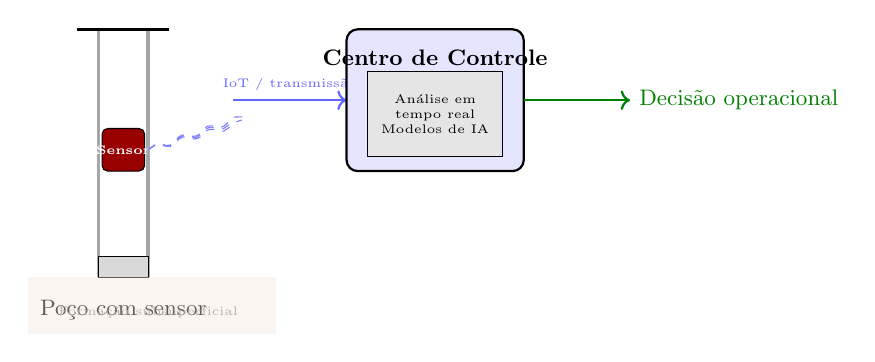
\begin{tikzpicture}[scale=0.9, transform shape]
    % Poço com sensor
    \draw[very thick, gray!70] (0.5,0) -- (0.5,3.5);
    \draw[very thick, gray!70] (1.2,0) -- (1.2,3.5);
    \draw[very thick] (0.2,3.5) -- (1.5,3.5);
    \draw[fill=gray!30] (0.5,0) rectangle (1.2,0.3);
    % Sensor no fundo do poço
    \draw[fill=red!60!black, rounded corners=2pt] (0.55,1.5) rectangle (1.15,2.1);
    \node[font=\tiny\bfseries, white] at (0.85,1.8) {Sensor};
    % Sinal de transmissão
    \foreach \r in {0.3, 0.6, 0.9}
      \draw[blue!50, thin, dashed, decoration={snake, amplitude=1pt}, decorate]
        (1.2,1.8) -- ++(1.2+\r*0.2, 0.3+\r*0.2);
    \draw[->, blue!60, thick] (2.4,2.5) -- (4.0,2.5)
      node[midway, above, font=\tiny] {IoT / transmissão};
    % Centro de controle
    \draw[fill=blue!10, rounded corners=4pt, thick] (4.0,1.5) rectangle (6.5,3.5);
    \node[font=\small\bfseries] at (5.25,3.1) {Centro de Controle};
    \draw[fill=gray!20] (4.3,1.7) rectangle (6.2,2.9);
    \node[font=\tiny, align=center] at (5.25,2.3)
      {Análise em\\tempo real\\Modelos de IA};
    % Seta para decisão
    \draw[->, thick, green!50!black] (6.5,2.5) -- (8.0,2.5)
      node[right, font=\small] {Decisão operacional};
    % Label do poço
    \node[below, font=\small] at (0.85,-0.2) {Poço com sensor};
    % Subsolo
    \fill[brown!20, opacity=0.4] (-0.5,-0.8) rectangle (3.0,0);
    \node[font=\tiny, gray!60] at (1.2,-0.5) {Formação subsuperficial};
  \end{tikzpicture}
  \caption{Arquitetura de monitoramento em tempo real: sensores permanentes instalados no fundo do poço transmitem continuamente dados de pressão, temperatura, vazão e composição para centros de controle onde algoritmos de análise identificam anomalias e oportunidades de otimização.}
  \label{fig:iot}
  \fonte{Elaboração própria.}
\end{figure}

A difusão da Internet das Coisas (IoT) e dos sensores de fundo de poço
de alta precisão revolucionou o monitoramento de campos petrolíferos.
Sensores permanentes transmitem, de forma contínua, medições de
pressão, temperatura, vazão e composição para centros de controle em
superfície (Figura~\ref{fig:iot}). Isso permite detectar precocemente
anomalias operacionais, identificar oportunidades de otimização e
calibrar modelos de reservatório de forma dinâmica — reduzindo a
incerteza e aumentando a eficiência do campo \cite{ramos2020}.

A integração desses dados com modelos de simulação em tempo real deu
origem aos chamados \textbf{reservatórios digitais} (\textit{digital
twins}): réplicas virtuais e permanentemente atualizadas dos campos
físicos, que permitem testar cenários de produção, antecipar falhas
e otimizar decisões operacionais sem interromper a produção.

% - - - - - - - - - - - - - - - - - - - - - - - - - - - - - -
\subsection{Modelagem Computacional Avançada e Sistemas de Suporte à Decisão}
% - - - - - - - - - - - - - - - - - - - - - - - - - - - - - -

Os modelos computacionais contemporâneos transcendem os simuladores
clássicos de diferenças finitas. A \textbf{Fluidodinâmica Computacional
(CFD)} simula em detalhe tridimensional o escoamento multifásico em
poços, tubulações e instalações de superfície, permitindo a otimização
do design de completação e o cálculo preciso de gradientes de pressão
em instalações submarinas de águas profundas.

Os \textbf{Sistemas de Suporte à Decisão (SSD)} integram dados de
produção histórica, modelos de reservatório e algoritmos de otimização
— como algoritmos genéticos, programação dinâmica e otimização
estocástica — para definir as melhores estratégias de alocação de
investimentos, sequenciamento de perfuração e otimização contínua da
produção. Esses sistemas introduzem rigor matemático onde antes havia
julgamento intuitivo \cite{ahmed2010, terry2015}.

% - - - - - - - - - - - - - - - - - - - - - - - - - - - - - -
\subsection{Inteligência Artificial e Aprendizado de Máquina}
% - - - - - - - - - - - - - - - - - - - - - - - - - - - - - -

% -------- FOTO: IA / Machine Learning em campo petrolífero --------
\begin{figure}[H]
  \centering
  % Substituir este fbox por \includegraphics[width=0.78\textwidth]{fotos/ia_reservatorio.png}
  \fbox{\parbox{0.78\textwidth}{\centering Representação visual de aplicação de Inteligência Artificial\\ em Engenharia de Reservatórios: redes neurais para previsão\\ de declínio de produção, ou interface de plataforma de\\ analítica avançada (SLB Delfi, Halliburton DecisionSpace 365).\\[4pt] \textbf{Sugestão:} ``Machine learning oil reservoir'' -- Unsplash / Pexels (licença gratuita) ou material educacional de fabricante de software}}
  \caption{Inteligência Artificial aplicada à Engenharia de Reservatórios: redes neurais e algoritmos de aprendizado de máquina permitem prever curvas de declínio, otimizar parâmetros de produção em tempo real e identificar padrões em dados sísmicos 4D com precisão e velocidade sem precedentes.}
  \label{fig:ia_reservatorio}
  \fonte{[INSERIR REFERÊNCIA DA IMAGEM REAL]}
\end{figure}

A segunda década do século XXI marcou a entrada consolidada das
técnicas de aprendizado de máquina e de Inteligência Artificial na
Engenharia de Reservatórios. A diferença fundamental em relação aos
modelos físicos clássicos é que os modelos de ML aprendem padrões
\textit{diretamente dos dados}, sem necessidade de especificação
explícita de todas as relações causais — o que os torna especialmente
poderosos quando a física do sistema é parcialmente desconhecida ou
excessivamente complexa.

As aplicações já consolidadas incluem: (i) previsão de declínio de
produção mediante redes neurais recorrentes; (ii) otimização em tempo
real de pressão de fundo de poço e razão de injeção de água; (iii)
caracterização petrofísica automatizada a partir de imagens digitais
de testemunho (\textit{digital rock physics}); (iv) identificação de
padrões em dados sísmicos 4D para monitoramento de frentes de fluido;
e (v) detecção precoce de anomalias em equipamentos de fundo de poço
\cite{ahmed2010, ramos2016}.

% - - - - - - - - - - - - - - - - - - - - - - - - - - - - - -
\subsection{Reservatórios Não Convencionais}
% - - - - - - - - - - - - - - - - - - - - - - - - - - - - - -

% FIGURA 8 – Reservatório não convencional (TikZ melhorado)
\begin{figure}[H]
  \centering
  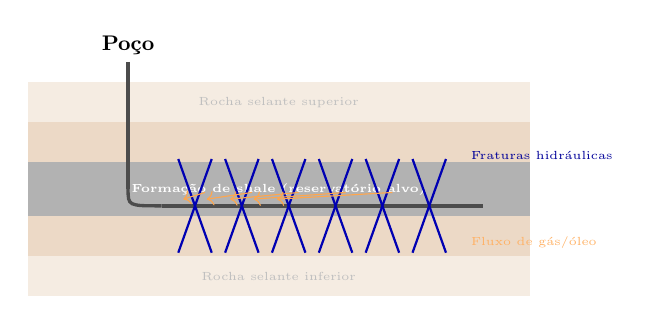
\begin{tikzpicture}[scale=0.85, transform shape]
    % Camadas geológicas
    \fill[brown!15] (0,0) rectangle (7.5,0.6);
    \fill[brown!30] (0,0.6) rectangle (7.5,1.2);
    \fill[gray!60] (0,1.2) rectangle (7.5,2.0);  % shale alvo
    \fill[brown!30] (0,2.0) rectangle (7.5,2.6);
    \fill[brown!15] (0,2.6) rectangle (7.5,3.2);
    % Labels de camadas
    \node[font=\tiny, gray!50] at (3.75,0.3) {Rocha selante inferior};
    \node[font=\tiny, white] at (3.75,1.6) {\textbf{Formação de shale (reservatório alvo)}};
    \node[font=\tiny, gray!50] at (3.75,2.9) {Rocha selante superior};
    % Poço vertical
    \draw[very thick, black!70] (1.5,3.5) -- (1.5,1.6);
    % Curva do poço horizontal
    \draw[very thick, black!70] (1.5,1.6) .. controls (1.5,1.35) .. (2.0,1.35);
    \draw[very thick, black!70] (2.0,1.35) -- (6.8,1.35);
    % Fraturas hidráulicas
    \foreach \x in {2.5, 3.2, 3.9, 4.6, 5.3, 6.0}
    {
      \draw[blue!70!black, thick] (\x,1.35) -- (\x+0.25, 2.05);
      \draw[blue!70!black, thick] (\x,1.35) -- (\x-0.25, 2.05);
      \draw[blue!70!black, thick] (\x,1.35) -- (\x+0.25, 0.65);
      \draw[blue!70!black, thick] (\x,1.35) -- (\x-0.25, 0.65);
    }
    % Setas de fluxo de gás
    \foreach \x in {2.65, 3.35, 4.05, 4.75, 5.45}
      \draw[->, orange!70, thin] (\x,1.55) -- ($(\x,1.55)!0.5!(2.0,1.35)$);
    % Labels
    \node[above, font=\small\bfseries] at (1.5,3.5) {Poço};
    \node[right, font=\tiny, blue!60!black] at (6.5,2.1) {Fraturas hidráulicas};
    \node[right, font=\tiny, orange!60] at (6.5,0.8) {Fluxo de gás/óleo};
  \end{tikzpicture}
  \caption{Esquema de poço horizontal com fraturas hidráulicas em reservatório de \textit{shale}: a rede de fraturas artificiais cria a permeabilidade necessária para viabilizar economicamente a produção em formações de ultra-baixa permeabilidade (nanodarcies).}
  \label{fig:shale}
  \fonte{Adaptado de \citeonline{javadpour2009}.}
\end{figure}

O \textit{shale boom} norte-americano, a partir de 2008, foi uma das
maiores revoluções energéticas da história recente. A combinação de
perfuração horizontal com fraturamento hidráulico em múltiplos estágios
tornou viável a produção em formações de argila orgânica com
permeabilidades da ordem de nanodarcies — absolutamente impensável
com técnicas convencionais \cite{javadpour2009}.

Mais do que uma revolução tecnológica, o \textit{shale} impôs novos
desafios teóricos: a Lei de Darcy clássica torna-se inadequada nessas
escalas, sendo necessário incorporar difusão de Knudsen, adsorção
molecular do metano nas paredes dos mesoporos e geomecânica acoplada.
A modelagem de reservatórios não convencionais continua sendo uma das
fronteiras mais ativas da pesquisa na área \cite{javadpour2009}.

% - - - - - - - - - - - - - - - - - - - - - - - - - - - - - -
\subsection{Gás Natural e a Engenharia de Reservatórios de Gás}
% - - - - - - - - - - - - - - - - - - - - - - - - - - - - - -

O crescimento do gás natural como combustível de transição energética
— menos intensivo em carbono que o óleo e o carvão — ampliou
significativamente o escopo da disciplina. Os reservatórios de gás
apresentam particularidades que exigem tratamento especializado:
o comportamento de gases reais descrito pelo fator $Z$, a formação de
hidratos em condições de alta pressão e baixa temperatura, e a gestão
de condensado retrógrado ao redor do poço. A obra de \cite{ramos2020}
constitui referência essencial para o tratamento aprofundado dessas
particularidades em língua portuguesa.

% - - - - - - - - - - - - - - - - - - - - - - - - - - - - - -
\subsection{\texorpdfstring{Captura e Armazenamento Geológico de CO\textsubscript{2}}{Captura e Armazenamento Geológico de CO2}}
% - - - - - - - - - - - - - - - - - - - - - - - - - - - - - -

% FIGURA 9 – CCS (TikZ melhorado)
\begin{figure}[H]
  \centering
  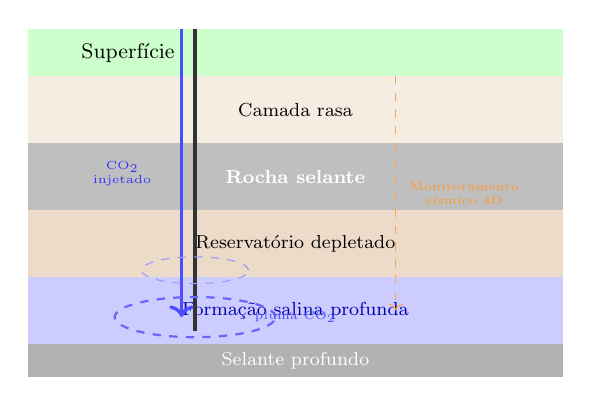
\begin{tikzpicture}[scale=0.85, transform shape]
    % Superfície
    \fill[green!20] (0,4.5) rectangle (8,5.2);
    \node[font=\small] at (1.5,4.85) {Superfície};
    % Camadas geológicas
    \fill[brown!15] (0,3.5) rectangle (8,4.5); % raso
    \fill[gray!50] (0,2.5) rectangle (8,3.5); % selante
    \fill[brown!35, opacity=0.8] (0,1.5) rectangle (8,2.5); % reserv.
    \fill[blue!20] (0,0.5) rectangle (8,1.5); % salino
    \fill[gray!60] (0,0) rectangle (8,0.5); % selante prof.
    % Labels
    \node[font=\footnotesize] at (4,4.0) {Camada rasa};
    \node[font=\footnotesize, white] at (4,3.0) {\textbf{Rocha selante}};
    \node[font=\footnotesize] at (4,2.0) {Reservatório depletado};
    \node[font=\footnotesize, blue!70!black] at (4,1.0)
      {Formação salina profunda};
    \node[font=\footnotesize, white] at (4,0.25) {Selante profundo};
    % Poço de injeção
    \draw[very thick, black!80] (2.5,5.2) -- (2.5,0.7);
    % CORREÇÃO: nó com quebra de linha usando text width e align
    \draw[->, very thick, blue!70] (2.3,5.2) -- (2.3,0.9)
      node[midway, left, font=\tiny, blue!80, text width=1.5cm, align=center] {CO$_2$\\injetado};
    % Pluma de CO2
    \draw[dashed, blue!60, thick] (2.5,0.9) ellipse (1.2 and 0.3);
    \draw[dashed, blue!40] (2.5,1.6) ellipse (0.8 and 0.2);
    \node[font=\tiny, blue!70] at (4.0,0.9) {pluma CO$_2$};
    % Seta de monitoramento sísmico - CORREÇÃO: nó com quebra de linha
    \draw[->, dashed, orange!70] (5.5,4.5) -- (5.5,1.0)
      node[midway, right, font=\tiny, orange!80, text width=1.8cm, align=center] {Monitoramento\\sísmico 4D};
  \end{tikzpicture}
  \caption{Esquema de Captura e Armazenamento Geológico de CO\textsubscript{2} (CCS): o CO\textsubscript{2} capturado é injetado em formações salinas profundas ou reservatórios depletados, com monitoramento sísmico 4D para verificar o confinamento da pluma ao longo de décadas.}
  \label{fig:ccs}
  \fonte{Adaptado de \citeonline{bachu2000}.}
\end{figure}

Uma das fronteiras mais promissoras e estratégicas da disciplina na
atualidade é a sua contribuição para as metas climáticas globais por
meio da Captura e Armazenamento de CO\textsubscript{2} (CCS). O
conhecimento acumulado em caracterização de reservatórios, modelagem
de escoamento multifásico e monitoramento sísmico está sendo
diretamente reaproveitado para o armazenamento permanente de
CO\textsubscript{2} em formações salinas profundas e em reservatórios
depletados \cite{bachu2000}.

No contexto angolano, a avaliação do potencial de campos maduros para
armazenamento geológico de CO\textsubscript{2} representa uma
oportunidade singular de diversificação técnica e de contribuição
tangível para os compromissos nacionais com os acordos climáticos
internacionais.

% - - - - - - - - - - - - - - - - - - - - - - - - - - - - - -
\subsection{Novas Fronteiras: Além do Petróleo Convencional}
% - - - - - - - - - - - - - - - - - - - - - - - - - - - - - -

Uma importante tendência contemporânea é a aplicação das metodologias
desenvolvidas na Engenharia de Reservatórios para novos domínios de
exploração e armazenamento no subsolo. Essa expansão não representa
o abandono da disciplina, mas sua evolução para responder aos desafios
energéticos e ambientais do século XXI \cite{terry2015}.

Três aplicações emergentes merecem destaque:

\begin{itemize}
  \item \textbf{Armazenamento de Hidrogénio Verde}: reservatórios depletados
    e formações salinas profundas podem armazenar hidrogénio produzido
    por eletrólise a partir de fontes renováveis, funcionando como
    ``baterias'' geológicas para a economia de hidrogénio. As técnicas
    de caracterização petrofísica e modelagem de escoamento aplicam-se
    diretamente;
  \item \textbf{Exploração de Energia Geotérmica Associada}: campos
    petrolíferos frequentemente possuem gradientes geotérmicos aproveitáveis
    para geração de eletricidade ou aquecimento direto. A compreensão
    do fluxo térmico em reservatórios, herdada da engenharia de petróleo,
    é fundamental;
  \item \textbf{Monitoramento Sísmico 4D para Sustentabilidade}: a tecnologia
    de sísmica repetida, inicialmente desenvolvida para rastreamento de
    injeção de água e gás em campos de petróleo, permite agora monitorar
    projetos de armazenamento de carbono, estabilidade de depósitos de
    resíduos, e até mesmo a integridade de estruturas geológicas em
    contextos de mitigação climática.
\end{itemize}

Esses desenvolvimentos indicam que a Engenharia de Reservatórios não é
uma disciplina em declínio — pelo contrário, ela está vivenciando um
renascimento como disciplina \textit{estratégica para a transição
energética global}. Os profissionais formados nessa área estarão bem
posicionados para papéis cruciais em empresas de energia renovável,
projetos de compensação carbônica, gestão de infraestrutura subterrânea,
e até em agências ambientais especializadas em monitoramento geológico.

\subsection{Captura e Armazenamento de CO\textsubscript{2} (CCS): Um Novo Paradigma}
% - - - - - - - - - - - - - - - - - - - - - - - - - - - - - -

Entre as aplicações emergentes, a \textbf{Captura e Armazenamento de
CO\textsubscript{2}} (CCS) merece atenção especial pela sua importância
estratégica na mitigação das mudanças climáticas. Neste caso, a
Engenharia de Reservatórios não extrai hidrocarbonetos, mas sim
\textit{armazena permanentemente} dióxido de carbono capturado em
fontes industriais ou atmosféricas.

O funcionamento de CCS segue princípios fundamentais herdados diretamente
da engenharia de exploração de petróleo. O CO\textsubscript{2} capturado
é comprimido, transportado e injetado em formações geológicas profundas
— tipicamente em depósitos salinos, reservatórios depletados de petróleo
ou gás, ou aquíferos profundos selados \cite{bachu2000}. Uma vez injetado,
o CO\textsubscript{2} permanece confinado pelos mesmos mecanismos que
aprisionaram hidrocarbonetos durante milhões de anos: um teto geológico
impermeável (folhelho, sal, argilito) e pressão litostática que mantém
o fluido injetado na profundidade \cite{ahmed2010}.

Os desafios técnicos de CCS são intimamente relacionados aos da
Engenharia de Reservatórios clássica:

\begin{itemize}
  \item \textbf{Caracterização e modelagem}: necessário mapear porosidade,
    permeabilidade e propriedades de confinamento com precisão, usando as
    mesmas técnicas petrofísicas e sísmicas empregadas em exploração de óleo;
  \item \textbf{Previsão de comportamento}: requer modelagem numérica de
    escoamento em meios porosos, análise de gradientes de pressão, e
    simulação de migração de CO\textsubscript{2};
  \item \textbf{Monitoramento a longo prazo}: emprega sísmica 4D e análise
    de pressão transiente para verificar a integridade do confinamento ao
    longo de décadas;
  \item \textbf{Remediação de anomalias}: se identificadas fugas ou migração
    indesejada, a expertise em controle de poços e injeção/produção é
    fundamental.
\end{itemize}

Para Angola, onde a indústria petrolífera permanece estratégica, o domínio
de tecnologias CCS representa uma oportunidade única de \textit{liderança
técnica regional}. Engenheiros angolanos capazes de projetar tanto a
exploração de reservatórios de hidrocarbonetos quanto de ``reservatórios
de carbono'' terão valor diferenciado no cenário energético pós-carbono.
Além disso, muitos campos maduros angolanos — que enfrentam declínio de
produção — poderiam ser repurposados como sítios de armazenamento de
carbono, gerando receita adicional e contribuindo para objetivos
internacionais de redução de emissões \cite{bachu2000}.

% -----------------------------------------------------------
\section{Desafios Atuais e Perspectivas Futuras da Engenharia de Reservatórios}
\label{sec:desafios_futuro}
% -----------------------------------------------------------

A Engenharia de Reservatórios, após mais de um século e meio de evolução
acelerada, enfrenta atualmente um conjunto de desafios complementares e
de perspectivas transformadoras que devem ocupar centralidade nas
estratégias de pesquisa e desenvolvimento para a próxima década
\cite{ahmed2010, terry2015}.

\subsection{Desafios Técnicos Contemporâneos}

O primeiro grande desafio reside na \textbf{maturidade dos campos
petrolíferos}. Muitos dos reservatórios em operação encontram-se em
fase avançada de exploração, apresentando declínio natural de pressão
e redução drástica de taxas de produção. Campos que produziram milhões
de barris diários em seu apogeu encontram-se frequentemente reduzidos
a dezenas de milhares. A aplicação de técnicas sofisticadas de EOR em
campos maduros é cada vez mais necessária, mas também economicamente
marginal, exigindo inovação nas próprias técnicas de recuperação para
reduzir custos operacionais \cite{lake2007}.

O segundo desafio é a \textbf{complexidade geológica crescente}. Os
campos de fácil exploração — estruturas simples, geometrias claras,
reservatórios homogêneos — foram na sua maioria já desenvolvidos.
A fronteira atual deslocou-se para ambientes de altíssima complexidade:
águas profundas e ultra-profundas descendo a 3 km ou mais, reservatórios
geologicamente fraturados e heterogêneos em múltiplas escalas,
formações de ultra-baixa permeabilidade (\textit{tight oil and gas},
\textit{shale}), depósitos de hidrocarbonetos em sedimentos conturbados
e estruturalmente complexos. Nesses ambientes, a caracterização do
reservatório torna-se extraordinariamente desafiadora: a sísmica
convencional é frequentemente insuficiente, e a geometria do campo
pode apresentar surpresas significativas durante a perfuração
\cite{ahmed2010}.

Um terceiro desafio é de natureza \textbf{ambiental e climática}. A
pressão regulatória e social para reduzir as emissões de carbono e os
impactos ambientais da exploração petrolífera impõe constrições crescentes
sobre a indústria. Já não é suficiente extrair petróleo — é preciso fazê-lo
com o menor dano ambiental possível, reduzindo gases de efeito estufa,
protegendo aquíferos de água doce, minimizando o descarte de fluidos de
produção. Essas exigências apresentam frequentemente soluções técnicas
incompatíveis: maximizar recuperação exige frequentemente técnicas que
aumentam o impacto ambiental. A resolução dessa tensão é um dos problemas
de engenharia mais sofisticados do período.

\subsection{Perspectivas Futuras: Transformação Digital e Além}

Apesar dos desafios, o horizonte futuro da Engenharia de Reservatórios
é extraordinariamente promissor, fundamentado em três eixos principais.

O primeiro eixo é a \textbf{transformação digital} estruturada. A
integração massiva de dados em tempo real (IoT), a modelagem avançada
e os algoritmos de aprendizado de máquina estão transformando a forma
como os engenheiros tomam decisões. Não se trata apenas de aplicar
automação aos processos existentes — trata-se de reimaginar completamente
a natureza da análise de reservatórios. Sistemas de gémeos digitais
(\textit{digital twins}) permitem que campos reais inteiros sejam
replicados em ambientes virtuais, onde cenários podem ser testados
instantaneamente, otimizações podem ser computadas continuamente, e
anomalias podem ser detectadas em tempo real. Esses avanços prometem
aumentar as taxas de recuperação e reduzir os custos operacionais de
forma substancial \cite{ramos2020}.

O segundo eixo é a \textbf{sustentabilidade como oportunidade técnica}.
A captura e armazenamento de carbono (CCS), conforme discutido, não é
uma simples aplicação de técnicas antigas a um novo fluido — é uma
aplicação da Engenharia de Reservatórios a um problema climático global.
A mesma disciplina que aprendeu a extrair petróleo pode agora aprender
a armazenar carbono de forma permanente e segura. Além disso, reservatórios
depletados podem ser convertidos em fontes de energia renovável via
armazenamento subterrâneo de ar comprimido ou energia térmica. Esses
desenvolvimentos alinham a Engenharia de Reservatórios com as metas
globais de transição energética \cite{bachu2000}.

O terceiro eixo é a \textbf{integração multidisciplinar}. O engenheiro
de reservatórios do futuro operará num contexto totalmente distinto do
seu predecessor do século XX. Será necessário dominar não apenas os
fundamentos clássicos de física e matemática dos reservatórios, mas
também processamento de dados em larga escala, algoritmos de
aprendizado de máquina, modelagem de sistemas climáticos, gestão
ambiental, economia de energia, e critério crítico sobre os impactos
sociais de decisões técnicas.

Essa multidisciplinaridade não é opcional — é imperativa. Um engenheiro
que domina perfeitamente as equações de escoamento multifásico mas é
analfabeto em Python e inteligência artificial será, no contexto de
2030, tão ineficaz quanto um engenheiro de 1900 que dominasse apenas
técnicas empíricas sem qualquer compreensão da Lei de Darcy. Do mesmo
modo, um engenheiro que compreenda dados e algoritmos mas careça de
sólida formação nos fundamentos físicos dos reservatórios estará fadado
a cometer erros sistemáticos e onerosos.

A formação para essa nova realidade requer currícula radicalmente
reimaginados que integrem essas múltiplas dimensões de forma coesa desde
o primeiro ano de estudos, não como disciplinas isoladas, mas como
componentes de uma visão sistêmica da gestão de recursos energéticos
no século XXI.

% -----------------------------------------------------------
\section{Síntese Histórica: Principais Marcos}
\label{sec:sintese}
% -----------------------------------------------------------

A Figura~\ref{fig:timeline} apresenta uma linha do tempo com os marcos
mais relevantes da evolução da disciplina, da formulação da Lei de
Darcy em 1856 à era digital do século XXI.

% FIGURA 10 – Linha do tempo (TikZ melhorado)
\begin{figure}[H]
  \centering
  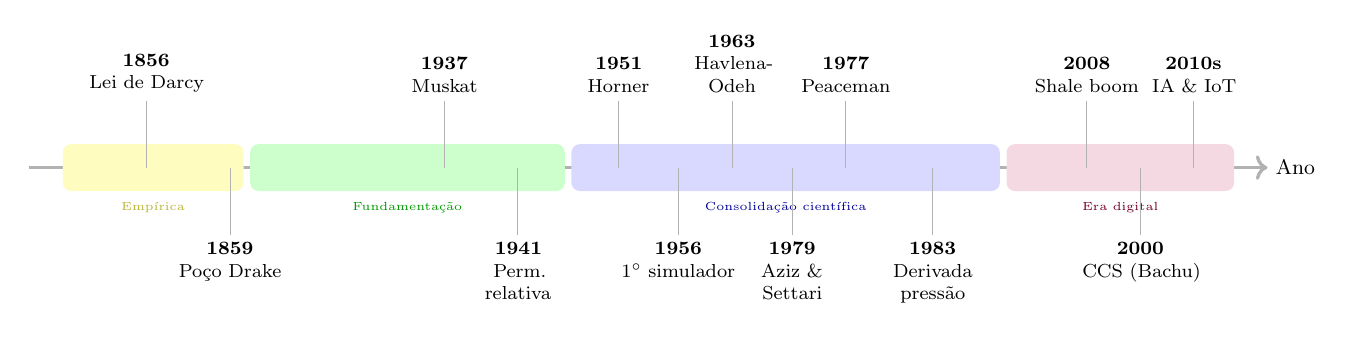
\begin{tikzpicture}[scale=0.85, transform shape, every node/.style={font=\footnotesize}]
    % Linha central
    \draw[->, very thick, gray!60] (0,0) -- (18.5,0);
    % Períodos coloridos
    \fill[yellow!25, rounded corners=3pt] (0.5,-0.35) rectangle (3.2,0.35);
    \fill[green!20, rounded corners=3pt] (3.3,-0.35) rectangle (8.0,0.35);
    \fill[blue!15, rounded corners=3pt] (8.1,-0.35) rectangle (14.5,0.35);
    \fill[purple!15, rounded corners=3pt] (14.6,-0.35) rectangle (18.0,0.35);
    % Labels de períodos
    \node[font=\tiny, yellow!70!black] at (1.85,-0.6) {Empírica};
    \node[font=\tiny, green!60!black] at (5.65,-0.6) {Fundamentação};
    \node[font=\tiny, blue!60!black] at (11.3,-0.6) {Consolidação científica};
    \node[font=\tiny, purple!60!black] at (16.3,-0.6) {Era digital};
    % Marcos (alternando acima e abaixo)
    % Acima
    \foreach \pos/\ano/\desc in {
      1.75/1856/Lei de Darcy,
      6.2/1937/Muskat,
      8.8/1951/Horner,
      10.5/1963/Havlena-Odeh,
      12.2/1977/Peaceman,
      15.8/2008/Shale boom,
      17.4/2010s/IA \& IoT
    }
    {
      \draw[gray!60, thin] (\pos,0) -- (\pos,1.0);
      \node[above, align=center, text width=1.8cm] at (\pos,1.0)
        {\textbf{\ano}\\\desc};
    }
    % Abaixo
    \foreach \pos/\ano/\desc in {
      3.0/1859/Poço Drake,
      7.3/1941/Perm.\ relativa,
      9.7/1956/1$^{\circ}$ simulador,
      11.4/1979/Aziz \& Settari,
      13.5/1983/Derivada pressão,
      16.6/2000/CCS (Bachu)
    }
    {
      \draw[gray!60, thin] (\pos,0) -- (\pos,-1.0);
      \node[below, align=center, text width=1.8cm] at (\pos,-1.0)
        {\textbf{\ano}\\\desc};
    }
    % Eixo temporal
    \node[right, font=\small] at (18.5,0) {Ano};
  \end{tikzpicture}
  \caption{Linha do tempo dos principais marcos históricos da Engenharia de Reservatórios de Petróleo: da fundamentação teórica clássica à era digital. As faixas coloridas demarcam as quatro eras paradigmáticas identificadas neste trabalho.}
  \label{fig:timeline}
  \fonte{Elaboração própria.}
\end{figure}

% Tabela de marcos históricos
\clearpage
\setlength{\tabcolsep}{2pt}
\renewcommand{\arraystretch}{1.2}
\begin{longtable}{p{1.8cm} p{5.0cm} p{5.2cm}}
\caption{Marcos históricos da Engenharia de Reservatórios de Petróleo}
\label{tab:marcos}\\
\toprule
\textbf{Período} & \textbf{Marco / Evento} & \textbf{Referência / Autor} \\
\midrule
\endfirsthead
\multicolumn{3}{l}{\small\itshape Continuação da Tabela~\ref{tab:marcos}}\\
\toprule
\textbf{Período} & \textbf{Marco / Evento} & \textbf{Referência / Autor} \\
\midrule
\endhead
\bottomrule
\endfoot
\bottomrule
\endlastfoot
\small
1856       & Lei de Darcy -- lei fundamental do escoamento em meios porosos & \cite{dake2014} \\
1859       & Poço Drake -- fundação da indústria petrolífera comercial & \cite{yergin1991} \\
1937--1949 & Sistematização matemática da E.R.\ por Muskat & \cite{muskat1949} \\
1941       & Permeabilidade relativa (Leverett \& Lewis) & \cite{rosa2006} \\
1947       & Correlações PVT de Standing & \cite{mccain1990} \\
1951       & Método de Horner para análise de \textit{buildup} & \cite{dake2014} \\
1963       & Balanço de materiais como relação linear (Havlena-Odeh) & \cite{havlena1963} \\
1977       & Fundamentos da simulação numérica de reservatórios (Peaceman) & \cite{peaceman1977} \\
1979       & Simulação por elementos finitos (Aziz \& Settari) & \cite{aziz1979} \\
1983       & Método da derivada de pressão em testes de poço (Bourdet) & \cite{bourdet1989} \\
1990       & Propriedades de fluidos petrolíferos (McCain) & \cite{mccain1990} \\
1991       & The Prize: História da indústria petrolífera (Yergin) & \cite{yergin1991} \\
1991       & Applied Petroleum Reservoir Engineering, 2.ª ed. (Craft et al.) & \cite{craft1991} \\
1994       & Fundamentals of Reservoir Engineering (Dake) & \cite{dake1994} \\
2000       & Armazenamento geológico de CO\textsubscript{2} (Bachu) & \cite{bachu2000} \\
2006       & Engenharia de Reservatórios de Petróleo (Rosa et al.) & \cite{rosa2006} \\
2007       & Enhanced Oil Recovery (Lake) & \cite{lake2007} \\
2008       & Boom do \textit{shale gas/oil} -- novos modelos de escoamento & \cite{javadpour2009} \\
2010       & Reservoir Engineering Handbook, 4.ª ed. (Ahmed) & \cite{ahmed2010} \\
2014       & The Practice of Reservoir Engineering, ed. rev. (Dake) & \cite{dake2014} \\
2015       & Applied Petroleum Reservoir Engineering, 3.ª ed. (Terry et al.) & \cite{terry2015} \\
2015       & Petroleum Engineering Handbook (SPE) & \cite{spe2015} \\
2016       & Fundamentos Computacionais em Eng. de Petróleo (Ramos) & \cite{ramos2016} \\
2019       & Propriedades Microscópicas de Rochas Reservatório (Alyafei) & \cite{alyafei2019} \\
2019       & Reservoir Simulation and Management (Mungan) & \cite{mungan2019} \\
2020       & Engenharia de Reservatórios: Métodos Analíticos e Computacionais (Ramos) & \cite{ramos2020} \\
2023       & Statistical Review of World Energy (BP) & \cite{bp2023} \\
2023       & Petroleum and Other Liquids (EIA) & \cite{eia2023} \\
\end{longtable}

% ============================================================
\chapter{Conclusão}
\label{chap:conclusao}
% ============================================================

Ao percorrer a trajetória da Engenharia de Reservatórios de Petróleo
desde as práticas artesanais da Mesopotâmia até os algoritmos de
aprendizado de máquina do século XXI, o que se revela não é apenas
uma história de progresso técnico — é uma história sobre como a
humanidade aprende a fazer perguntas cada vez melhores sobre o mundo
que a rodeia.

A trajetória percorrida revela cinco rupturas paradigmáticas
fundamentais que merecem ser destacadas. A primeira foi a
\textbf{Lei de Darcy} (1856): antes dela, o engenheiro de campo
operava por instinto e experiência; depois dela, passou a ter uma
linguagem matemática precisa para descrever o que se passava no
subsolo. A segunda foi o \textbf{poço Drake} (1859): demonstrou que
extrair petróleo de forma controlada era possível e viável, abrindo
um ciclo de inovação sem precedentes. A terceira foi a
\textbf{sistematização matemática} de Muskat (1937; 1949): a
experiência acumulada de campo foi transformada em teoria rigorosa de
mecanismos de produção. A quarta foi a \textbf{simulação
computacional} (décadas de 1960--1980): permitiu modelar reservatórios
tridimensionais heterogêneos multifásicos, ampliando radicalmente o
horizonte de previsão disponível ao engenheiro. A quinta e mais
recente é a \textbf{integração entre modelagem física e inteligência
artificial}, que promete transformar novamente a natureza do trabalho
de engenharia de reservatórios nas próximas décadas
\cite{dake2014, yergin1991, peaceman1977, ramos2020}.

No contexto angolano, essas conclusões têm implicações práticas e
urgentes. Angola, como segundo maior produtor petrolífero da África
subsaariana, tem no domínio técnico da Engenharia de Reservatórios
não apenas um imperativo econômico, mas uma condição de soberania
energética. A crescente maturidade dos campos do bloco offshore e o
desenvolvimento de novas descobertas em águas ultra-profundas exigem
profissionais capazes de aplicar as metodologias mais avançadas de
caracterização, simulação e otimização de reservatórios. A formação
oferecida pelo ISPTEC — apoiada especialmente nas obras de
\cite{ramos2016} e \cite{ramos2020}, que articulam os fundamentos
clássicos com as ferramentas computacionais contemporâneas no contexto
lusófono — é um pilar fundamental dessa capacidade técnica nacional.

Para fortalecer ainda mais essa formação, recomendam-se as seguintes
diretrizes:

\begin{enumerate}[label=\roman*.]
  \item \textbf{Integração curricular da ciência de dados}: incorporar
    de forma estruturada as técnicas de aprendizado de máquina e de
    análise de grandes volumes de dados nos currículos de Engenharia
    de Petróleo, articulando-as com os fundamentos físicos clássicos;
  \item \textbf{Parcerias com operadores nacionais e internacionais}:
    estimular acordos de cooperação técnica e científica entre o ISPTEC
    e os principais operadores presentes em Angola, visando ao acesso
    a dados reais de campo para fins didáticos e de investigação;
  \item \textbf{Investigação em reservatórios angolanos}: desenvolver
    linhas de pesquisa dedicadas às especificidades dos reservatórios
    angolanos — carbonatos do pré-sal, turbiditos do pós-sal e
    potencial de armazenamento de CO\textsubscript{2} em campos
    maduros —, contribuindo para o conhecimento científico regional;
  \item \textbf{Fortalecimento da publicação científica lusófona}:
    incentivar a produção e publicação de obras de referência e de
    artigos científicos em língua portuguesa, à semelhança das
    contribuições pioneiras de \cite{rosa2006}, \cite{ramos2016}
    e \cite{ramos2020}.
\end{enumerate}

Em síntese, a Engenharia de Reservatórios de Petróleo permanece uma
disciplina viva e em constante transformação. Compreendê-la
historicamente é compreender, em miniatura, a própria essência da
engenharia: a aplicação metódica e criativa do conhecimento humano
para resolver problemas reais, complexos e frequentemente contraditórios.

A evolução descrita neste trabalho — do empirismo artesanal para a
ciência quantitativa, da análise retrospectiva para a previsão
prospectiva, da especialização focada para a multidisciplinaridade
integrada — não é meramente histórica: é profundamente contemporânea.
O engenheiro de reservatórios do século XXI não é mais alguém que domina
exclusivamente as técnicas de fluxo de fluidos em meios porosos. É,
necessariamente, um cientista de dados, um especialista em sustentabilidade,
um gestor de tecnologia, e um pensador crítico sobre as implicações
socioambientais de suas decisões técnicas.

Neste contexto de transformação, a Engenharia de Reservatórios está
expandindo suas fronteiras para novos domínios: armazenamento geológico
de CO\textsubscript{2} para compensação climática, produção de hidrogênio
verde em depósitos depletados, exploração de energia geotérmica associada
a reservatórios, e detecção de anomalias sísmicas para monitoramento
ambiental. Cada uma dessas aplicações demanda dos profissionais um
conhecimento cada vez mais integrado entre engenharia tradicional,
ciência dos dados, geociências, e responsabilidade ambiental.

Em Angola especificamente, onde os recursos naturais do subsolo são a
chave do desenvolvimento nacional — representando mais de 90\% das
exportações e a principal fonte de receitas fiscais — a capacitação de
engenheiros capazes de dominar essa disciplina em toda sua complexidade
contemporânea é não apenas um imperativo académico, mas uma necessidade
estratégica da mais alta ordem. A formação oferecida pela instituição
— alicerçada nos fundamentos históricos aqui discutidos e nas
ferramentas computacionais contemporâneas — é determinante para que
Angola possa exercer sua soberania técnica, garantir a eficiência
operacional de seus campos, e alinhar sua indústria energética com
as metas globais de transição sustentável.

Este trabalho investigativo, ao reconstruir a história da Engenharia de
Reservatórios, contribui para essa formação ao mostrar não apenas \textit{o quê}
a disciplina é hoje, mas \textit{como} chegou a ser dessa forma, quais
foram as rupturas paradigmáticas que a moldaram, e por que cada passo
dessa evolução permanece relevante para as decisões técnicas e
estratégicas do presente.

\postextual

% ------------------- REFERÊNCIAS BIBLIOGRÁFICAS -------------------
\bibliography{referencias}

\end{document}